%%%%%%%%%%%%%%%%%%%%%%%%%%%%%%%%%%%%%%%%%%%%%%%
%%% Template for lab reports used at STIMA
%%%%%%%%%%%%%%%%%%%%%%%%%%%%%%%%%%%%%%%%%%%%%%%

%%%%%%%%%%%%%%%%%%%%%%%%%%%%%% Sets the document class for the document
% Openany is added to remove the book style of starting every new chapter on an odd page (not needed for reports)
\documentclass[10pt,english, openany]{book}

%%%%%%%%%%%%%%%%%%%%%%%%%%%%%% Loading packages that alter the style
\usepackage{graphicx}
\usepackage{subcaption}
\usepackage[]{color}
\usepackage{alltt}
\usepackage[T1]{fontenc}
\usepackage[utf8]{inputenc}
\usepackage{amsfonts}
\usepackage{mathtools}
\setcounter{secnumdepth}{2}
\setcounter{tocdepth}{2}
\setlength{\parskip}{\smallskipamount}
\setlength{\parindent}{0pt}

% Set page margins
\usepackage[top=100pt,bottom=100pt,left=68pt,right=66pt]{geometry}

% Prevents LaTeX from filling out a page to the bottom
\raggedbottom

% Adding both languages
\usepackage[english, italian]{babel}

% All page numbers positioned at the bottom of the page
\usepackage{fancyhdr}
\fancyhf{} % clear all header and footers
\fancyfoot[C]{\thepage}
\renewcommand{\headrulewidth}{0pt} % remove the header rule
\pagestyle{fancy}

% Changes the style of chapter headings
%\usepackage{titlesec}
% \usepackage[Glenn]{fncychap}
% Adds table captions above the table per default
\usepackage{float}
\floatstyle{plaintop}
\restylefloat{table}

% Adds space between caption and table
\usepackage[tableposition=top]{caption}

% Adds hyperlinks to references and ToC
\usepackage{cite}
\usepackage{hyperref}
\hypersetup{hidelinks,linkcolor = black} % Changes the link color to black and hides the hideous red border that usually is created

% If multiple images are to be added, a folder (path) with all the images can be added here 
\graphicspath{ {Figures/} }

% Algorithms
\usepackage[ruled,vlined]{algorithm2e}

% Definitions
\usepackage{bm}
\usepackage{amsmath}
\newcommand{\myM}[1]{\bm{\mathit{#1}}} %Bold, italic, capital expression of matrices; vectors bold, italic, small
\newtheorem{definition}{Definition}
\DeclarePairedDelimiter\abs{\lvert}{\rvert}



% Separates the first part of the report/thesis in Roman numerals
\frontmatter
%%%%%%%%%%%%%%%%%%%%%%%%%%%%%% Starts the document
\begin{document}

%%% Selects the language to be used for the first couple of pages
\selectlanguage{english}

\author{Julian Eßer}
\title{Personal Lecture Notes \\
MITx6.832x: Underactuated Robotics \\
(Spring 2019) \\
{\Large Algorithms for Walking, Running, Swimming, Flying, and Manipulation}}

%%%%% Adds the title page
\begin{titlepage}
\maketitle
\end{titlepage}

% Adds a table of contents
\tableofcontents{}

%%%%%%%%%%%%%%%%%%%%%%%%%%%%%%%%%%%%%%%%%%%%%%%%%%%%%%%%%%%%%%%%%%%%%%%%%%%%%%%%%%%%%%%%%%%%
%%%%%%%%%%%%%%%%%%%%%%%%%%%%%%%%%%%%%%%%%%%%%%%%%%%%%%%%%%%%%%%%%%%%%%%%%%%%%%%%%%%%%%%%%%%%
%%%%% Text body starts here!
\mainmatter

\chapter{Introduction}\label{chapt:intro}
The purpose of this document is to provide a brief overview of the essential knowledge of the underactuated robotics class \cite{mitx6.832web} from MIT taught in Spring 2019. Special emphasis is on the following topics:\\
\begin{itemize}
\item Understanding Control as Optimization
\item Dynamics of Biped Locomotion
\item Optimization of Biped Locomotion
\end{itemize}

\chapter{CROCODDYL - LAAS-CNRS}\label{chapter1}
\section{Introduction}
\subsection{Motivation}
Crocoddyl is an \textbf{optimal control library for robot control under contact sequence}. Its solver is based on an efficient Differential Dynamic Programming (DDP) algorithm. Crocoddyl computes optimal trajectories along with optimal feedback gains. It uses Pinocchio for fast computation of robot dynamics and its analytical derivatives \cite{crocoddylweb}. 

Crocoddyl is focused on multi-contact optimal control problem (MCOP) which has the form:

$$\mathbf{X}^*,\mathbf{U}^*=
\begin{Bmatrix} \mathbf{x}^*_0,\cdots,\mathbf{x}^*_N \\
				  \mathbf{u}^*_0,\cdots,\mathbf{u}^*_N
\end{Bmatrix} =
\arg\min_{\mathbf{X},\mathbf{U}} \sum_{k=1}^N \int_{t_k}^{t_k+\Delta t} l(\mathbf{x},\mathbf{u})dt$$
subject to
$$ \mathbf{\dot{x}} = \mathbf{f}(\mathbf{x},\mathbf{u}),$$
$$ \mathbf{x}\in\mathcal{X}, \mathbf{u}\in\mathcal{U}, \boldsymbol{\lambda}\in\mathcal{K}.$$
where
\begin{itemize}
\item the state $\mathbf{x}=(\mathbf{q},\mathbf{v})$ lies in a manifold, e.g. Lie manifold $\mathbf{q}\in SE(3)\times \mathbb{R}^{n_j}$, $n_j$ being the number of degrees of freedom of the robot.
\item the system has underactuacted dynamics, i.e. $\mathbf{u}=(\mathbf{0},\boldsymbol{\tau})$,
\item $\mathcal{X}$, $\mathcal{U}$ are the state and control admissible sets, and
\item $\mathcal{K}$ represents the contact constraints.
\end{itemize}

Note that $\boldsymbol{\lambda}=\mathbf{g}(\mathbf{x},\mathbf{u})$ denotes the contact force, and is dependent on the state and control.

\subsection{Features}
According to the description in the Github repository \cite{crocoddylweb}, it comprises the following features:

Crocoddyl is \textbf{versatible}:
\begin{itemize}
\item various optimal control solvers (DDP, FDDP, BoxDDP, etc) - single and multi-shooting methods
\item analytical and sparse derivatives via Pinocchio
\item Euclidian and non-Euclidian geometry friendly via Pinocchio
\item handle autonomous and nonautomous dynamical systems
\item numerical differentiation support
\end{itemize}

Crocoddyl is \textbf{efficient} and \textbf{flexible}:
\begin{itemize}
\item cache friendly,
\item multi-thread friendly
\item Python bindings (including models and solvers abstractions)
\item C++ 98/11/14/17/20 compliant
\item extensively tested
\end{itemize}



\section{How-To}
\subsection{Install}
\subsubsection{Two ways to go}
Basically there are existing two ways of installing Crocoddyl: 
\begin{itemize}
\item Option 1: Installation via the \textit{robotpkg } package manager
\item Option 2: Installation from source
\end{itemize} 
I personally would recommend the installation through \textit{robotpkg}, since it preserves you from dealing with the multiple dependencies of Crocoddyl and therefore seems to be the faster approach. Generally you should decide beforehand which python version you want to use. This effects the robotpkg version as well as the export of the PYTHONPATH variable. 

\subsubsection{Installation via robotpkg (preferred)}
Steps for installing via robotpkg according to the installation section of \cite{crocoddylweb}
\begin{enumerate}
	\item Add robotpkg as source repository to apt:
	\begin{verbatim}
	sudo tee /etc/apt/sources.list.d/robotpkg.list <<EOF
	deb [arch=amd64] http://robotpkg.openrobots.org/wip/packages/debian/pub $(lsb_release -sc) robotpkg
	deb [arch=amd64] http://robotpkg.openrobots.org/packages/debian/pub $(lsb_release -sc) robotpkg
	EOF
	\end{verbatim}
	\item Register the authentication certificate of robotpkg:
	\begin{verbatim}
	curl http://robotpkg.openrobots.org/packages/debian/robotpkg.key | sudo apt-key add -
	\end{verbatim}
	\item You need to run at least once apt update to fetch the package descriptions:
	\begin{verbatim}
	sudo apt-get update
	\end{verbatim}
	\item The installation of Crocoddyl:
	\begin{verbatim}
	sudo apt install robotpkg-py27-crocoddyl # for Python 2
	sudo apt install robotpkg-py36-crocoddyl # for Python 3
	\end{verbatim}
	\item Finally you will need to configure your environment variables (watch out for the python version!), e.g.:
	\begin{verbatim}
	export PATH=/opt/openrobots/bin:$PATH
	export PKG_CONFIG_PATH=/opt/openrobots/lib/pkgconfig:$PKG_CONFIG_PATH
	export LD_LIBRARY_PATH=/opt/openrobots/lib:$LD_LIBRARY_PATH
	export PYTHONPATH=/opt/openrobots/lib/python3.6/site-packages:$PYTHONPATH
	\end{verbatim}
\end{enumerate}

\subsubsection{(Installation from source)}
If you prefer installing Crocoddyl from source, the following steps should do the work:
\begin{verbatim}
git clone https://github.com/loco-3d/crocoddyl.git 
git submodule update --init
mkdir build && cd build
export PKG_CONFIG_PATH=/opt/openrobots/lib/pkgconfig
cmake -DCMAKE_INSTALL_PREFIX=/opt/openrobots  ..
make
sudo make install
\end{verbatim}
Additionally you will have to install the dependent libraries (i.e. pinocchio, example-robot-data (optional for examples, install Python loaders), gepetto-viewer-corba (optional for display), jupyter (optional for notebooks) and matplotlib (optional for examples) and fix the incude paths.

\subsubsection{For Displaying Results: Additionally Install Gepetto-Viewer}
In order to see not just 2-dimensional plots, but also observe the 3D robot behaviour, you additionally have to install the gepetto-viewer.
\begin{verbatim}
 sudo apt install robotpkg-py36-qt4-gepetto-viewer-corba
\end{verbatim}

\subsection{Running the Examples}
Since the installation through robotpkg did not provide you with the examples from the git repository, you should clone the repo \cite{crocoddylweb} for getting the data. You do not have to build the library, since it already is installed. 
In the cloned repository go to \textit{/examples}. For running e.g. the bipedal walking example, just type
\begin{verbatim}
python3 bipedal_walk.py
\end{verbatim}
and you will see the calculations for optimal gait trajectories running in the console. 
The examples provide a \textit{plot} and \textit{display} argument. In order to display the 3D results and also plot some data, just do 
\begin{verbatim}
gepetto-gui
\end{verbatim}
for starting the 3D environment.
Then, in another terminal, run the example:
\begin{verbatim}
python3 bipedal_walk.py display plot
\end{verbatim}



\section{Abstract Workflow}
For each node (i.e. each timestep) of the optimal control problem, 
\begin{enumerate}
\item Load robot data (URDF, SRDF, Meshes)
\item Define Action Models (Dynamics+Costs) for running and terminal states 
	\begin{itemize}
	\item Setup a cost model
	\item Add the desired cost functions (state, control, frame-placement etc.)
	\item Calculate Integrated \& Differential Action Model (IAM/DAM) based on the model
	\end{itemize}
\item Define the optimal control problem (knots+IAMs, initPose)
\item Solve the Shooting Problem
\end{enumerate}



\section{Issues and Insights}
\subsection{Issues Encountered}
Since Crocoddyl currently is under active development, there frequently will occure smaller incompatibilities because of versioning issues.This is a brief overview of emerged difficulties:
\begin{itemize}
\item Python versioning errors in the examples. 

The examples most often are written for python2, which means that if you are under python3, you will have to adapt some commands (e.g. lists handling, matplotlib, print).
\item Crocoddyl versioning errors in the examples. 

Since Crocoddyl depends on other libraries (i.e. Pinnochio, example\_robot\_data), there sometimes occured errors with the class because they were not updated. 
\item Confusions displaying the results via the Gepetto-Viewer

The Gepetto-Viewer is used for displaying the robots and resulting trajectories from optimization. The examples only contain out of the box solutions. If one wants to simply display a robot in some specified pose (e.g. the initial pose) the following, quite unintuitive, commands have to be applied:
\begin{verbatim}
display = crocoddyl.GepettoDisplay(rh5_legs, 4, 4, frameNames=[rightFoot, leftFoot])
display.display(xs=[x0])
\end{verbatim}
\end{itemize}

\subsection{Cost Functions}
Notes:
\begin{itemize}
\item The cost function can contain multiple \textit{cost items} (i.e state/control error, frame displacements or center of mass tracking).
\item Weights are considered in the costs via scalar multiplication with the identity matrices (Ix, Ixx etc.) of the according cost item. 
\item These weighted matrices of cost items are simply summed up within a \textit{costModelContainer}.
\end{itemize}

\subsection{Joint Limits}
\begin{itemize}
\item Input Data: Within the URDF file, for each joint there are specified the
\begin{itemize}
	\item torque limit (effort),
	\item position limits (lower, upper),
	\item velocity limit.
\end{itemize}
\item These limits are not automatically taken into account in Crocoddyl when solving a shooting problem, but explicitly have to be adressed.
\item \textbf{Torque Limits}: Require the use of specific solvers, standard ddp is not sufficient. Implemented solvers that can handle torque limits explicitly are: 
\begin{itemize}
\item BoxDDP (Compare Tassa method \cite{tassa2014control})
\item BoxFDDP (Novel solver that is under development at LAAS)
\end{itemize}
\textbf{State Limits (Pos/Vel)}: Position and Velocity limits can be handled via penalization, i.e. added as cost terms to the optimization problem.  
\end{itemize}

\subsection{Introduction: Bipedal Walking in Crocoddyl}
\begin{itemize}
\item A long walk consists of multiple gaitphases, each phase is a single shooting problem.
\item These problems are generated with \textit{createWalkingProblem()} involving one left and one right foot step.
\item Each shooting problem contains various locomotion phases
	\begin{itemize}
	\item Double support at beginning (both legs on ground) via \textit{createSwingFootModel()}
	\item Right step (Swing-up and swing-down phase equally distributed) init via    	\textit{createFootstepModels()}
	\item Double support again
	\item Left step
	\end{itemize}	
\item In the end, all knots of all phases are basically one \textit{swingFootModel}. They only vary in the adressed foot, and if a CoM task or a swingFootTask is set.
\item The \textit{swingFootModel} is an IAM containing a 
	\begin{itemize}
	\item 6D multi-contact model,
	\item Cost model (CoM position tracking, contact friction cone, foot placement) and
	\item Differentiation (DAM) and Integration (IAM) routines.
	\end{itemize}
\end{itemize}

\subsection{Multi-Contact Model}
\subsubsection{Previous: Assume foot to have a point contact}
\begin{itemize}
\item Each \textit{swingFootModel}, meaning each knot of the OC, includes at least one individual contact model.
\item The number of contact models depends is specified via \textit{supportFootIds}, i.e. the number of foots that currently are not in the air (e.g. biped: 1 for swing-phase, 2 for double-support).
\item For each point of one foot that actually does touch the ground, a contact has to be added to the according contact model (specified via frame ID)
\item In the bipedal examples they assume a point-contact, i.e. adding only one contact per supporting foot.
\item The point-contact is specified via the name of the according link from the URDF.
\end{itemize}
\subsubsection{Extension: Consider 4 point contact per foot}
\begin{itemize}
\item Each contact model for one supporting foot now contains four contact items instead of one
\item The cost model contains now four cost items for the four friction cones instead of just one

\item The 
\end{itemize}



\section{Working with the Examples}
This section contains a brief overview of some of the examples that have been modified. Please note that many \textbf{additional explanations have been added in the commentaries of the examples}. All figures and additionaly videos are contained within the /media directory of the repo \cite{julesserOCFrameworks}. 

As stated in the ReadMe of the Repo, Crocoddyl comes with some introductory examples that are written as Jupyter notebooks (.ipynb). While 
\begin{verbatim}
examples/notebooks/introduction_to_crocoddyl.ipynb
\end{verbatim}
offers a more conceptual overview about crocoddyl, other ones represent basic underactuated systems (e.g. Cartpole swing-up, Bipdeal Walking).

\subsection{Manipulator: Multi-Point Trajectory}
The task in the tutorial
\begin{verbatim}
examples/notebooks/arm_manipulation.ipynb
\end{verbatim}
was to find an optimal trajectory for a manipulator from an initial configuration to a target point (red ball). 
\subsubsection{Extending the Example}
I extended this example to a multi-point optimal control problem by considering four targets to reach in a row. This extended example can be found in 
\begin{verbatim}
/examples/arm_manipulation_trajectory.py
\end{verbatim}
Differences to the existing one-target example include:
\begin{itemize}
\item Defining an array of the four targets in space
\item Setup individual cost functions for each of the sequences
\item Setup running and terminal models for the sequences and finally
\item Define the shooting problem as row of these sequences 
\item Optimize the weights of the cost functions successively for the four sequences.
\end{itemize}
\subsubsection{Results: Multiple Targets}
\begin{figure}[h!]
\centering
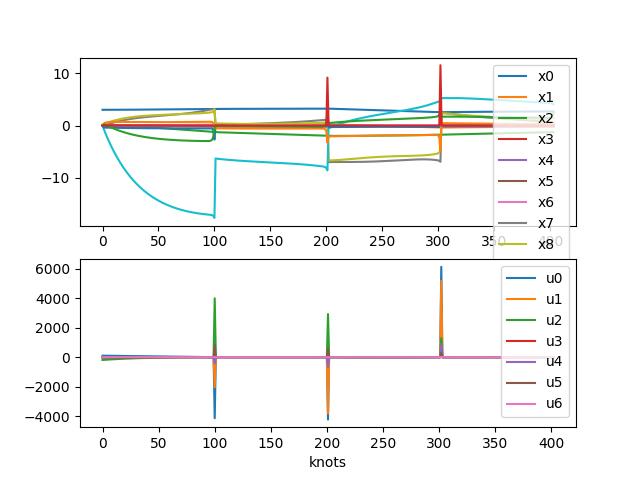
\includegraphics[width=.5\linewidth]{Media/Crocoddyl/ExArm/ArmSolution.png}
\caption{Multi-Point Optimal Control of the Manipulator for reaching four targets. The high-control peaks could be handled by a more advanced solver (e.g. box-ddp), but were not performed here.}
\end{figure}

\subsection{Talos Legs: Bipedal Walking}
The Crocoddyl library offers an example for bipedal walking with the lower body of the Talos \cite{stasse2017talos} Robot. The results of the solved trajectory can be found in Figure \ref{fig:TalosGait}. 

\begin{figure}[h!]
\centering
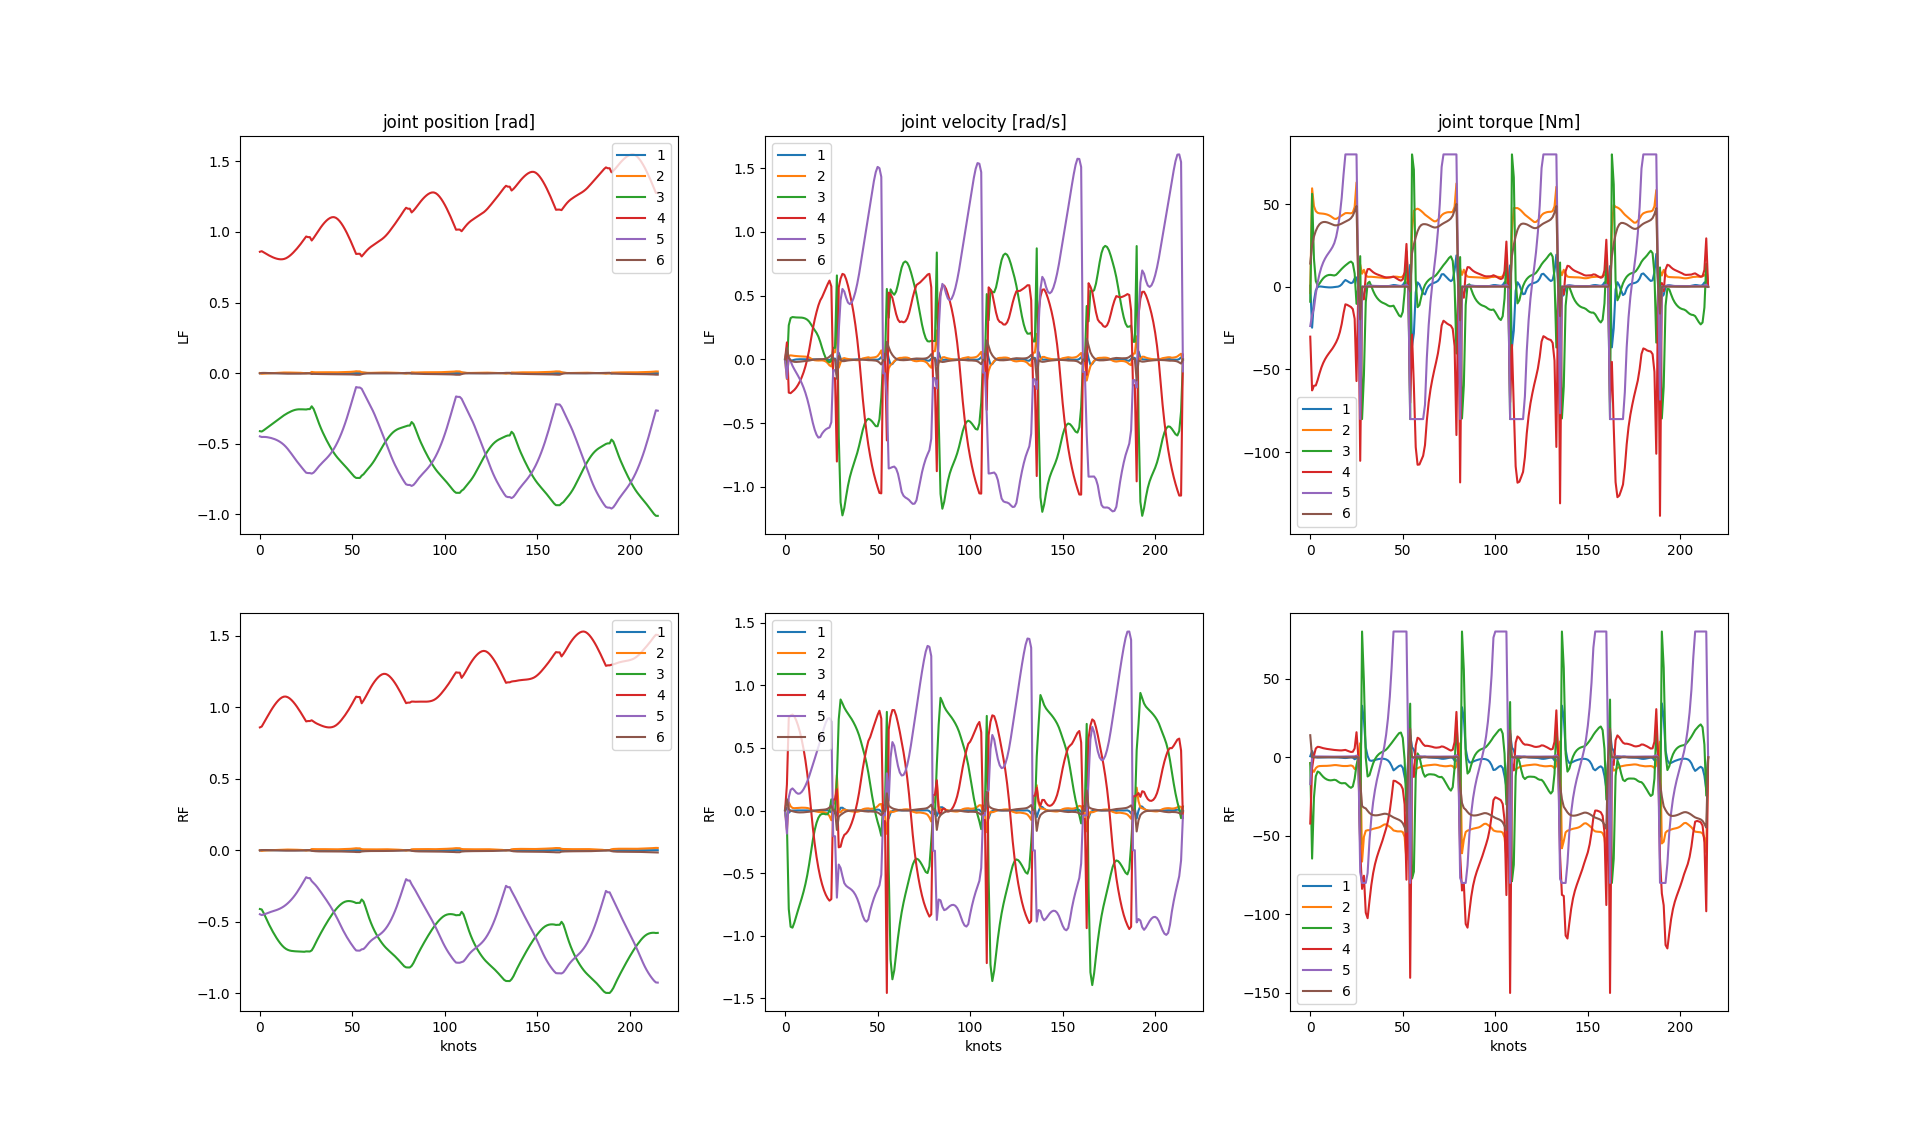
\includegraphics[width=.7\linewidth]{Media/Crocoddyl/ExBiped/TalosGait_Solution.png}
\caption{Results for a walk with three gait-phases.}
\label{fig:TalosGait}
\end{figure}

  



\section{RH5 Results}
Please note once again that all related plots and additional videos can be found in high-quality in the related github repository \cite{julesserOCFrameworks} of this project.
\subsection{Navigating the Files}
The main file for testing RH5 offers several options for setting up, analyzing and constraining the optimization problem of bipedal walking including
\begin{itemize}
\item Choosing a desired URDF 
\item Specifying gait length and variations in step length/height
\item Vary the initial pose of the robot
\item Constraining the torque input (Use different solver)
\item Defining singular or multiple point contacts per foot (Use different class from biped utils)
\end{itemize}

\subsection{Integration of the RH5 Legs into Crocoddyl}
The main issue that had to be solved was related to the underlying URDF file of the robot. In particular: 
\begin{itemize}
\item Choosing one of our several files (abstract-smurf)
\item Cutting out everything apart from the legs and the root joint
\item Fixing the mesh file paths: 

We usually define the path relative to the URDF file location, e.g.
\begin{verbatim}
"../meshes/stl/RH5_Root_Link.001.stl".
\end{verbatim}
The integrated URDF parser in Crocoddyl instead, expects the path specified via the package URI, e.g. 
\begin{verbatim}
"package://abstract-smurf/meshes/stl/RH5_Root_Link.001.stl".
\end{verbatim}
\item Adjust the contact frames for the Walking Problem.
\end{itemize}

\subsection{Performing two Steps}
Results are shown in Figure \ref{fig:rh5_two_steps}.
\begin{figure}[h!]
\centering
\begin{subfigure}{.4\textwidth}
  \centering
  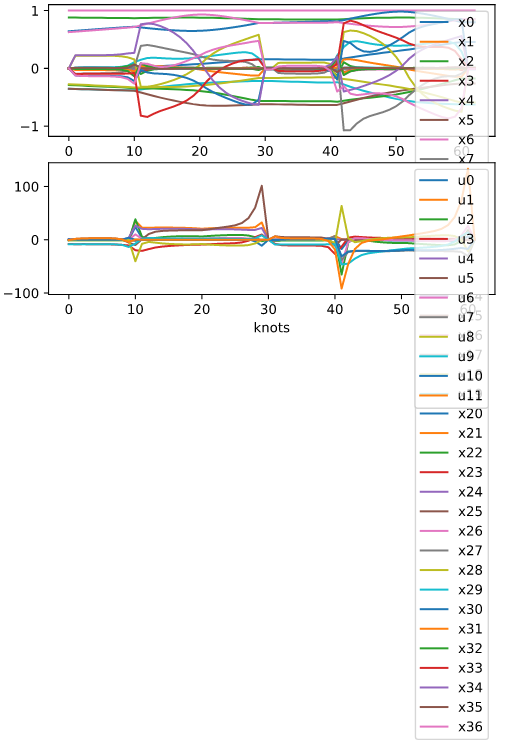
\includegraphics[width=1\linewidth]{Media/Crocoddyl/RH5/2Steps/RH52Steps_Solution.png}
  \caption{Optimal Trajectory and Conrol Inputs}
\end{subfigure}%
\begin{subfigure}{.4\textwidth}
  \centering
  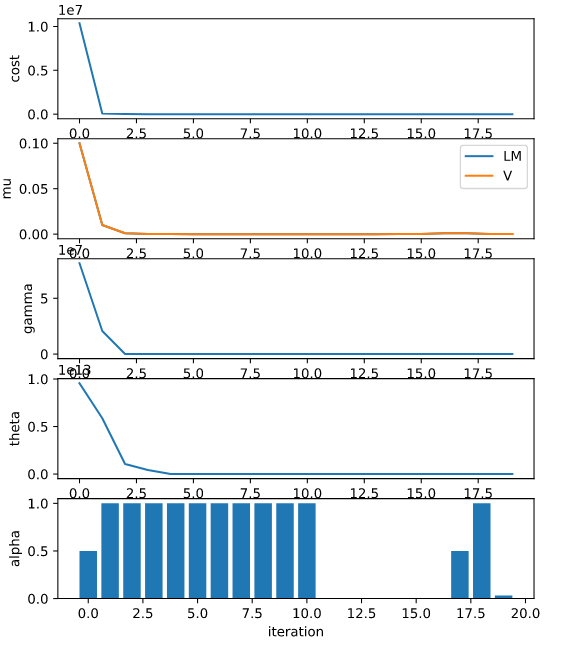
\includegraphics[width=1\linewidth]{Media/Crocoddyl/RH5/2Steps/RH52Steps_Convergence.png}
  \caption{Convergence of Solution}
\end{subfigure}
\caption{Results for a solved shooting problem defining two steps.}
\label{fig:rh5_two_steps}
\centering
\end{figure}

\subsection{Performing a Full Gait}
Results for a full gait (6 consecutive steps) are shown in Figure \ref{fig:rh5_full_gait}.
\begin{figure}[h!]
\centering
\begin{subfigure}{.8\textwidth}
  \centering
  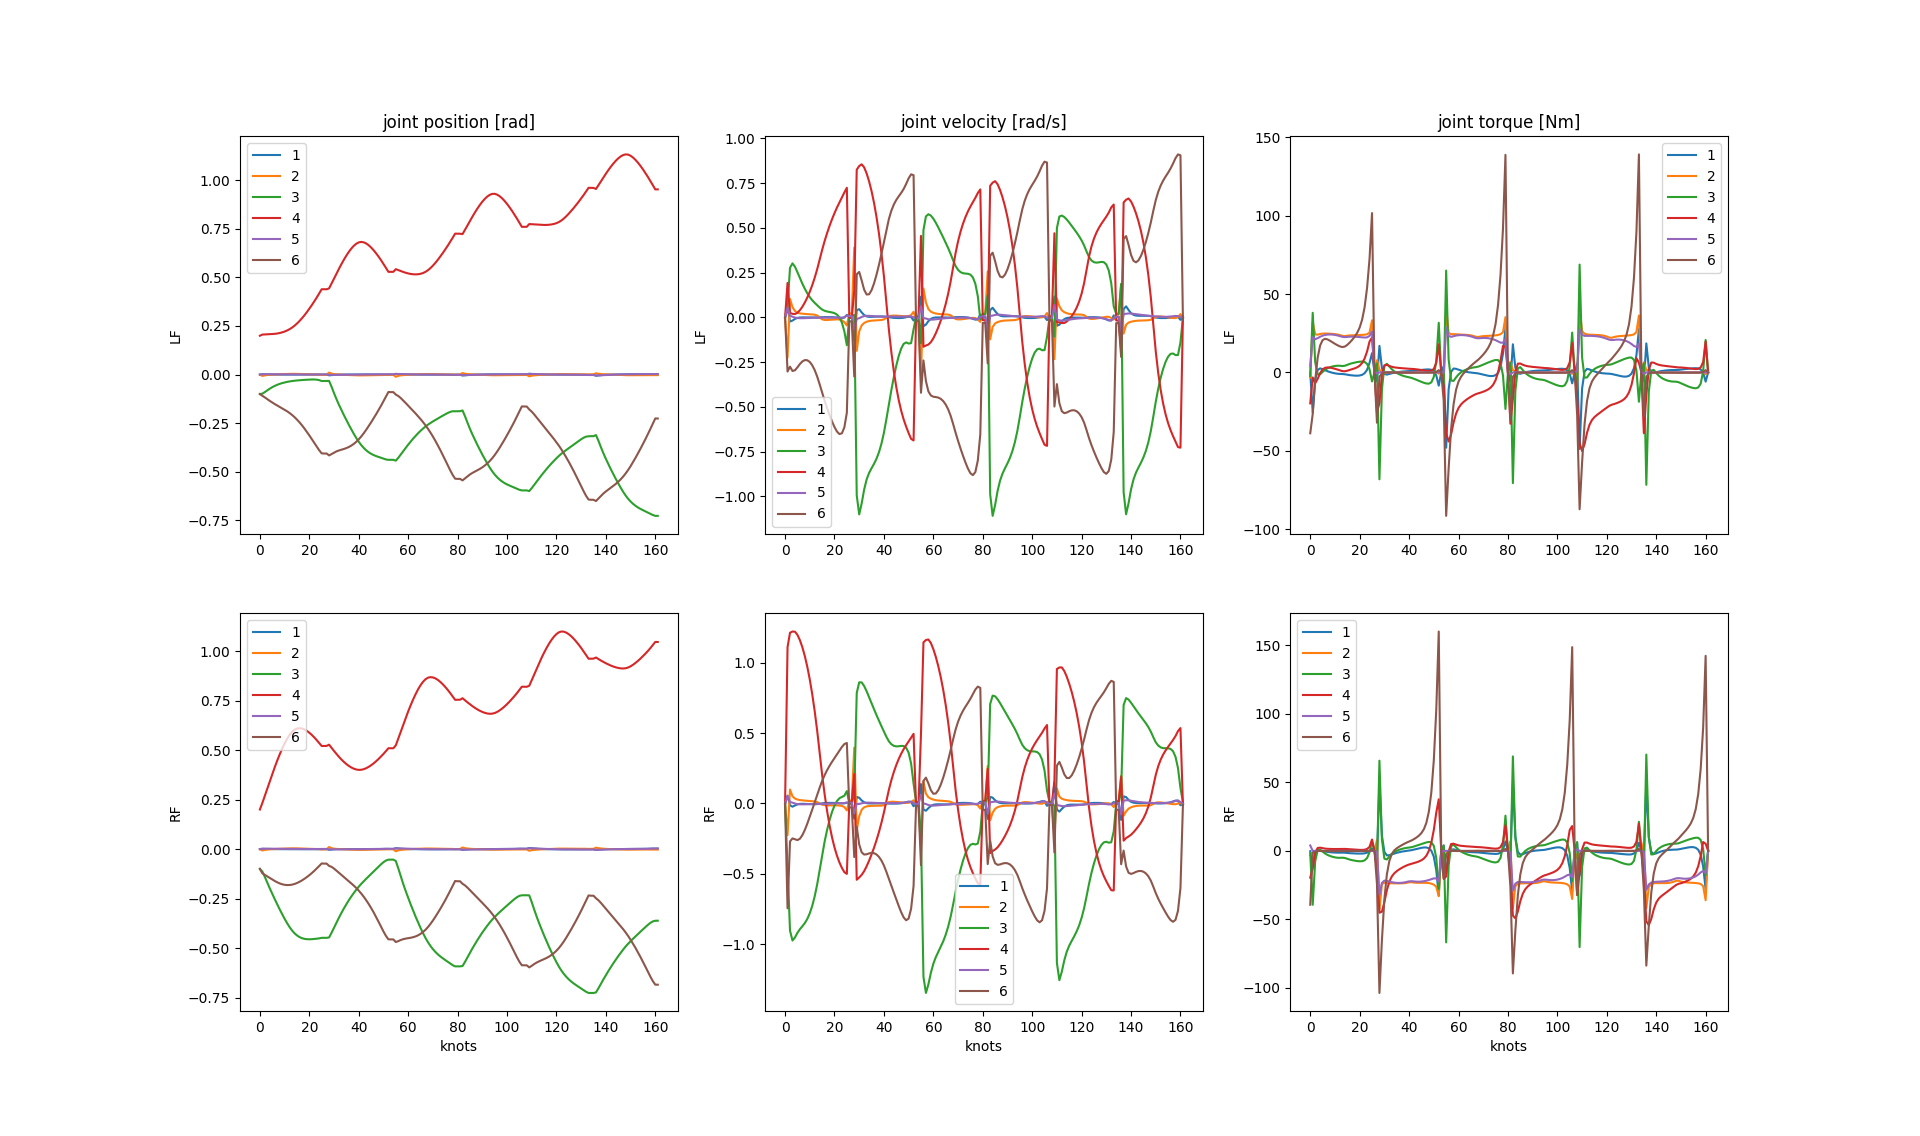
\includegraphics[width=1\linewidth]{Media/Crocoddyl/RH5/RH5Gait_Solution.png}
  \caption{Solution for states and torques.}
\end{subfigure}
\begin{subfigure}{.8\textwidth}
  \centering
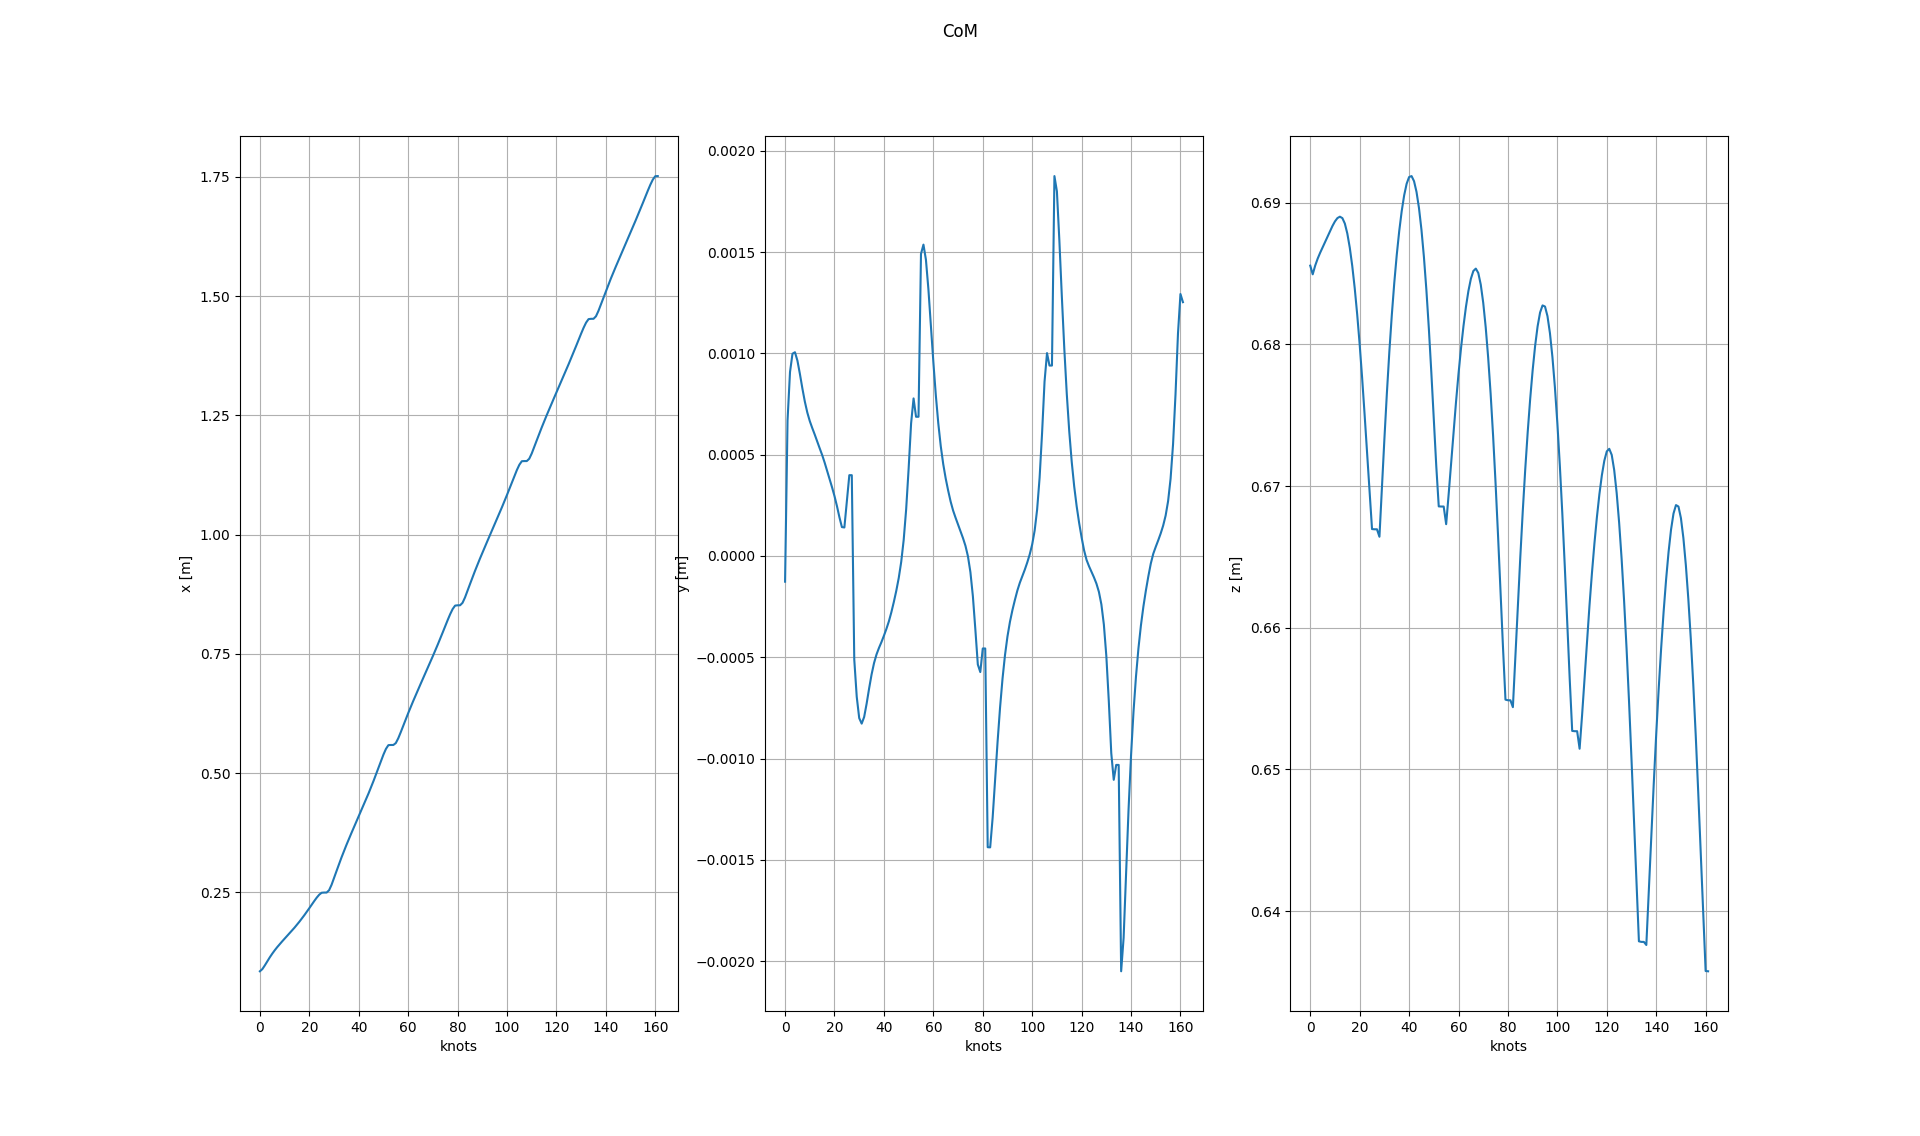
\includegraphics[width=1\linewidth]{Media/Crocoddyl/RH5/RH5Gait_CoM.png}
\caption{CoM results.}
\end{subfigure}
\caption{Results for a walk with three gait-phases. The walk is implemented as a sequence of three  consecutive shooting problems similar to the 2 steps task.}
\label{fig:rh5_full_gait}
\centering
\end{figure}

\subsection{Torque-Constrained Full Gait}
It is possible to constrain the input torques via the limits that are parsed from the URDF. However, the correct solver (box-ddp) needs to be applied to the OC problem for considering these limits.  Results are shown in Figure \ref{fig:rh5_constrain_torque}
\begin{figure}[h!]
\centering
\begin{subfigure}{.8\textwidth}
  \centering
  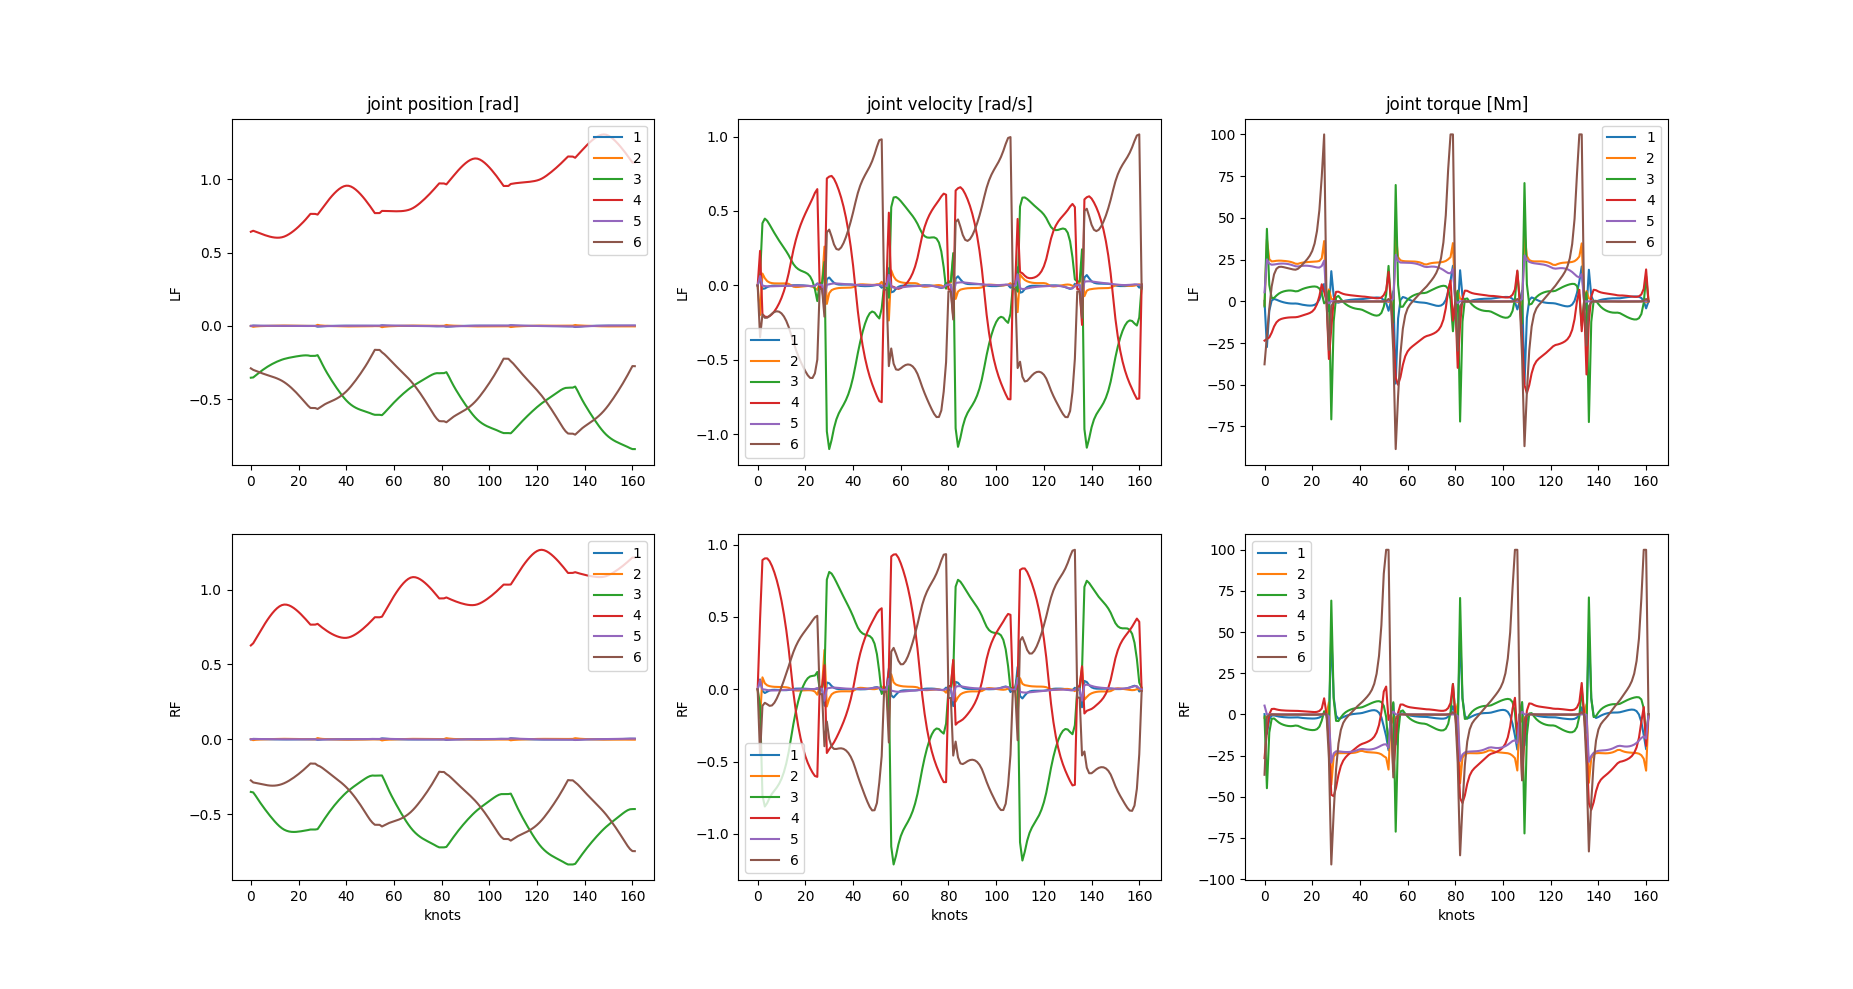
\includegraphics[width=1\linewidth]{Media/Crocoddyl/RH5/RH5GaitUbound50Percent_Solution.png}
  \caption{Solution for states and torques.}
\end{subfigure}
\begin{subfigure}{.8\textwidth}
  \centering
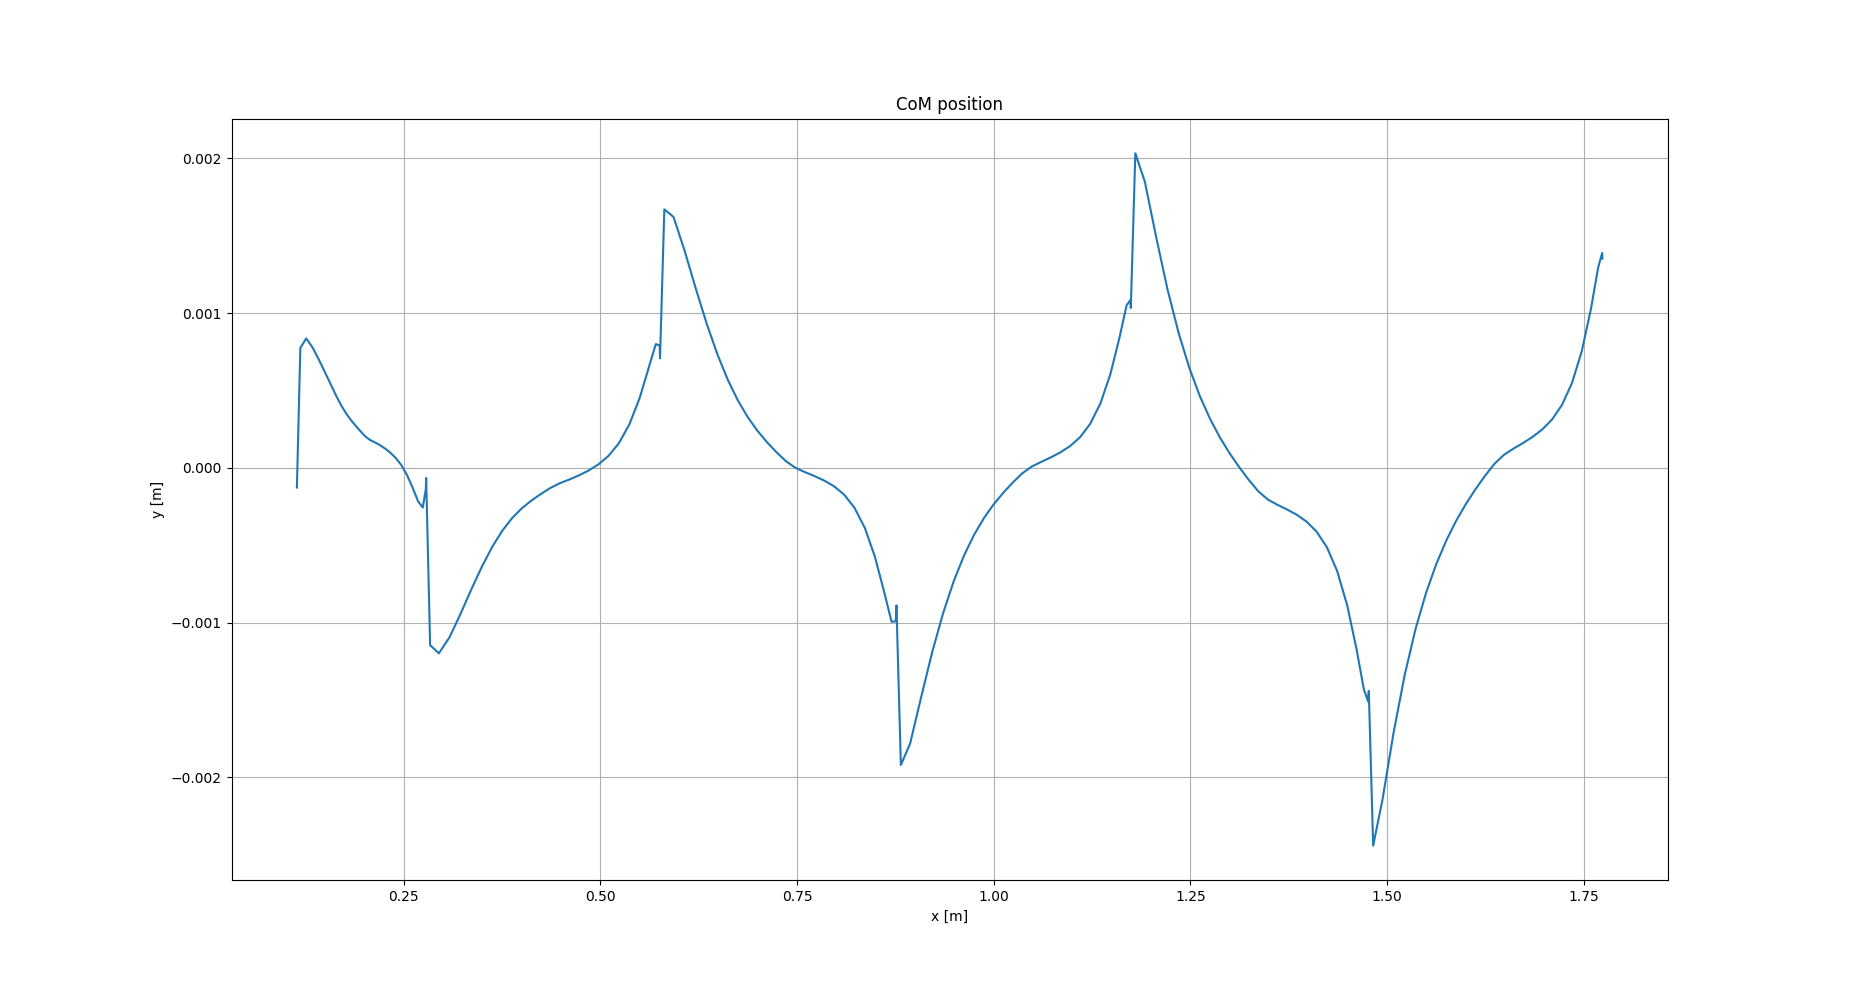
\includegraphics[width=1\linewidth]{Media/Crocoddyl/RH5/RH5GaitUbound50Percent_CoM.png}
\caption{CoM results.}
\end{subfigure}
\caption{Results for full gait with bounded input torques. To be even more restrictive, the available torques form the URDF have been reduced artificially by 50 percent. The effect becomes clear for e.g. the AnkleFT.}
\label{fig:rh5_constrain_torque}
\centering
\end{figure}

\subsection{Initial Pose Variants: Starting Near the Zero Configuration}
The full gait has been initialized according to the pose specifications from the RH5 DFKI smurf file. In this and the following section, two solutions for other initial poses are presented: One near the zero configuration and one at the zero configuration.

\begin{figure}[h!]
\centering
\begin{subfigure}{.8\textwidth}
  \centering
  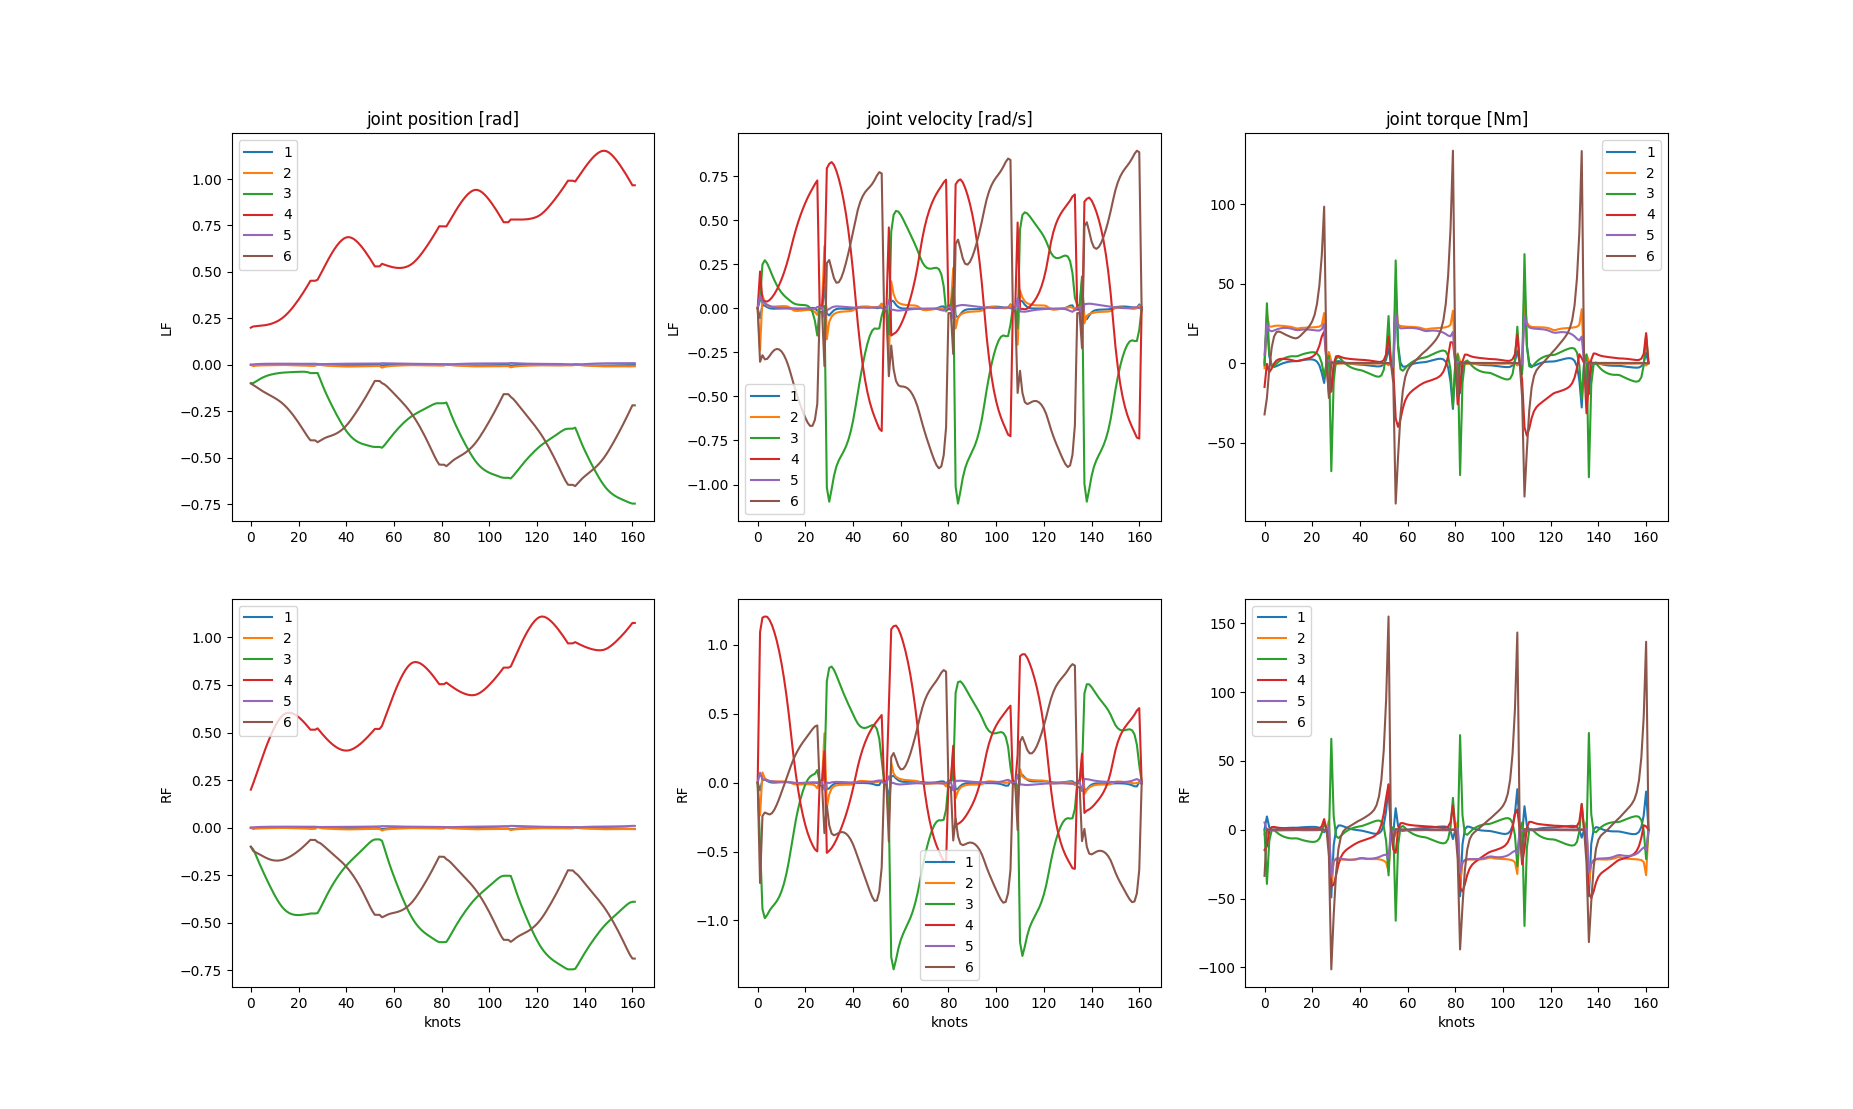
\includegraphics[width=1\linewidth]{Media/Crocoddyl/RH5/InitPoseVariants/RH5GaitInitNearZeroConfig_Solution.png}
  \caption{Solution for states and torques}.
\end{subfigure}
\begin{subfigure}{.8\textwidth}
  \centering
  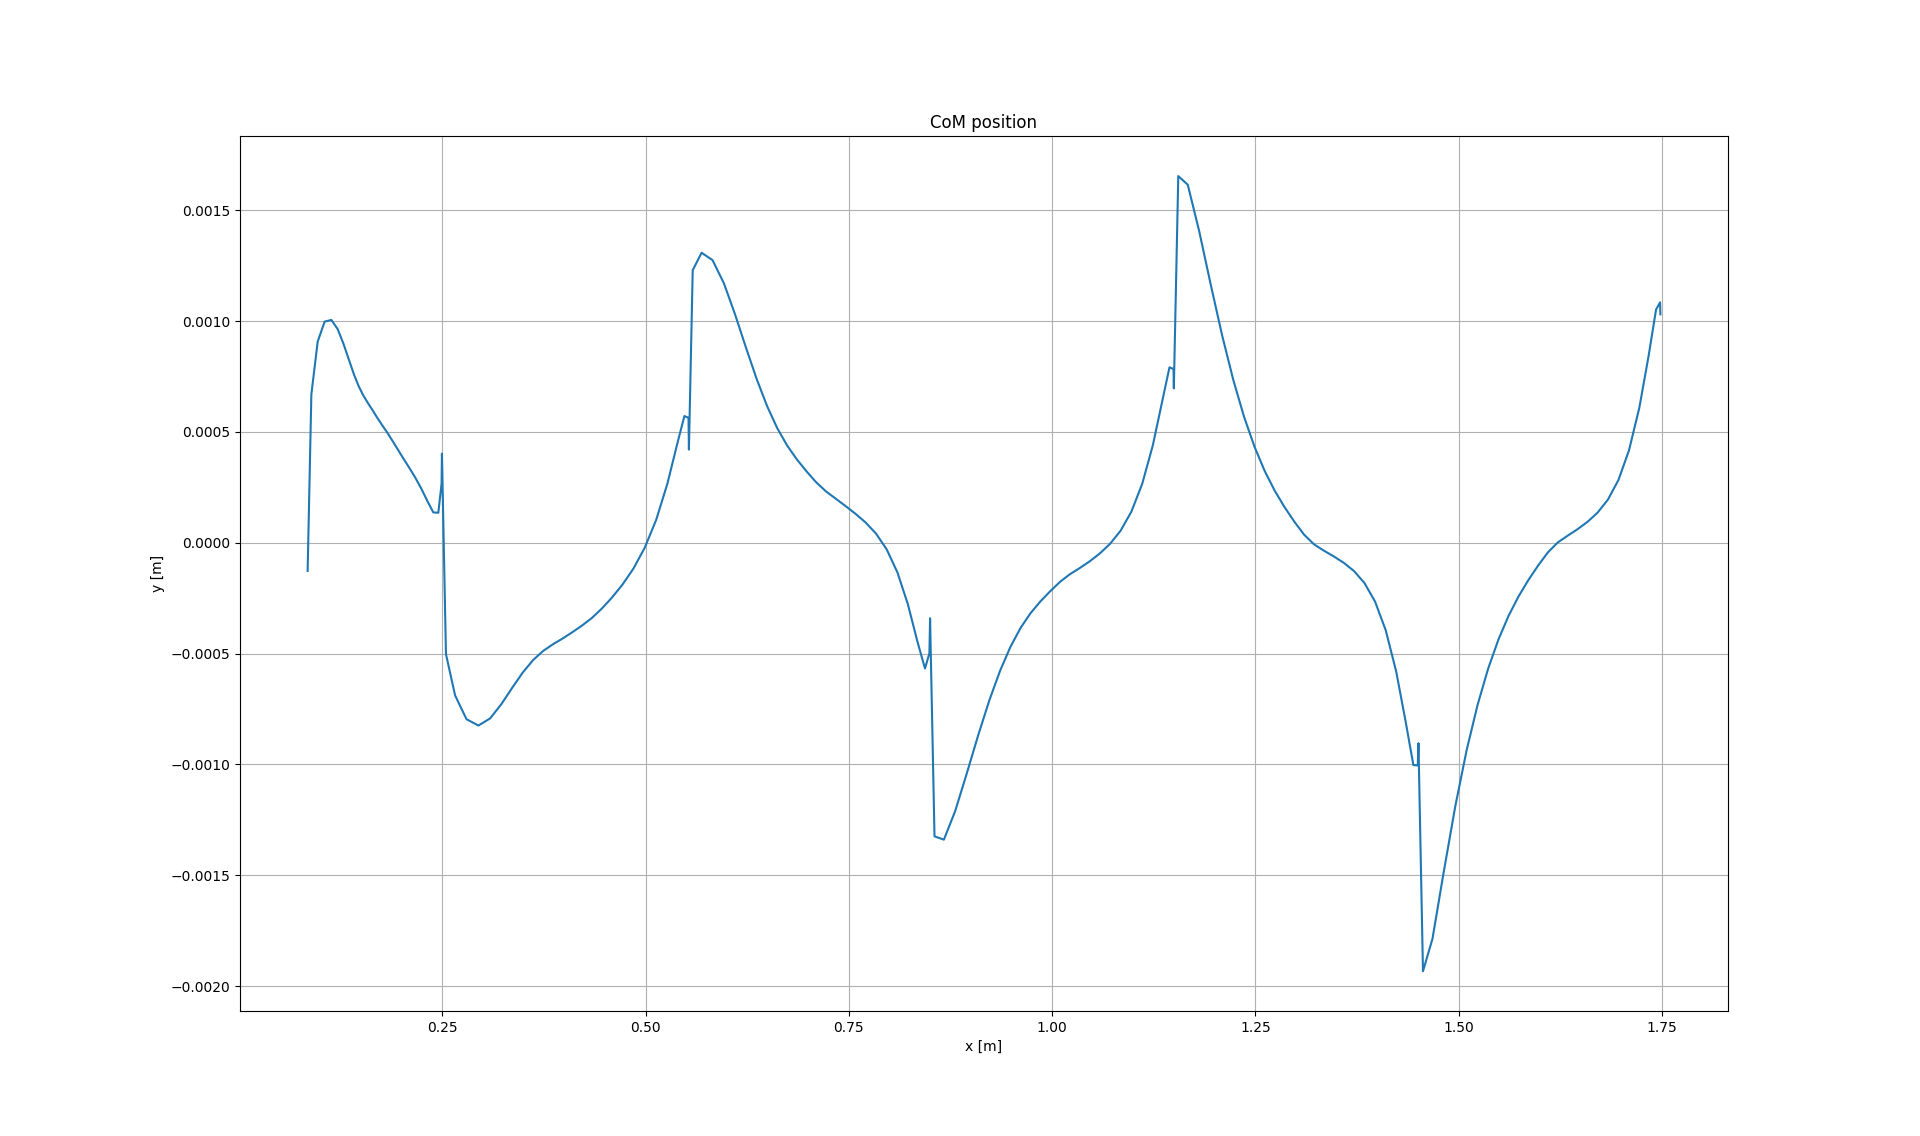
\includegraphics[width=1\linewidth]{Media/Crocoddyl/RH5/InitPoseVariants/RH5GaitInitNearZeroConfig_CoM.png}
\caption{CoM results.}
\end{subfigure}
\caption{Results for the full gait with initial pose \textbf{near} the zero configuration. q0=[0,0,-0.1,0.2,0,-0.1, 0,0,-0.1,0.2,0,-0.1] where  n=12 and represents the joint angles [rad] for the left and right leg.}
\label{fig:rh5_init_near_zero}
\centering
\end{figure}

\subsection{Initial Pose Variants: Starting At the Zero Configuration}
Initializing at the zero configuration turns out to be more critical. Sometimes the solver converges to a feasable solution (Figure \ref{fig:rh5_init_at_zero}), sometimes it does not find a proper solution (Figure \ref{fig:rh5_init_at_zero_failed_solver}).
\begin{figure}[h!]
\centering
\begin{subfigure}{.8\textwidth}
  \centering
  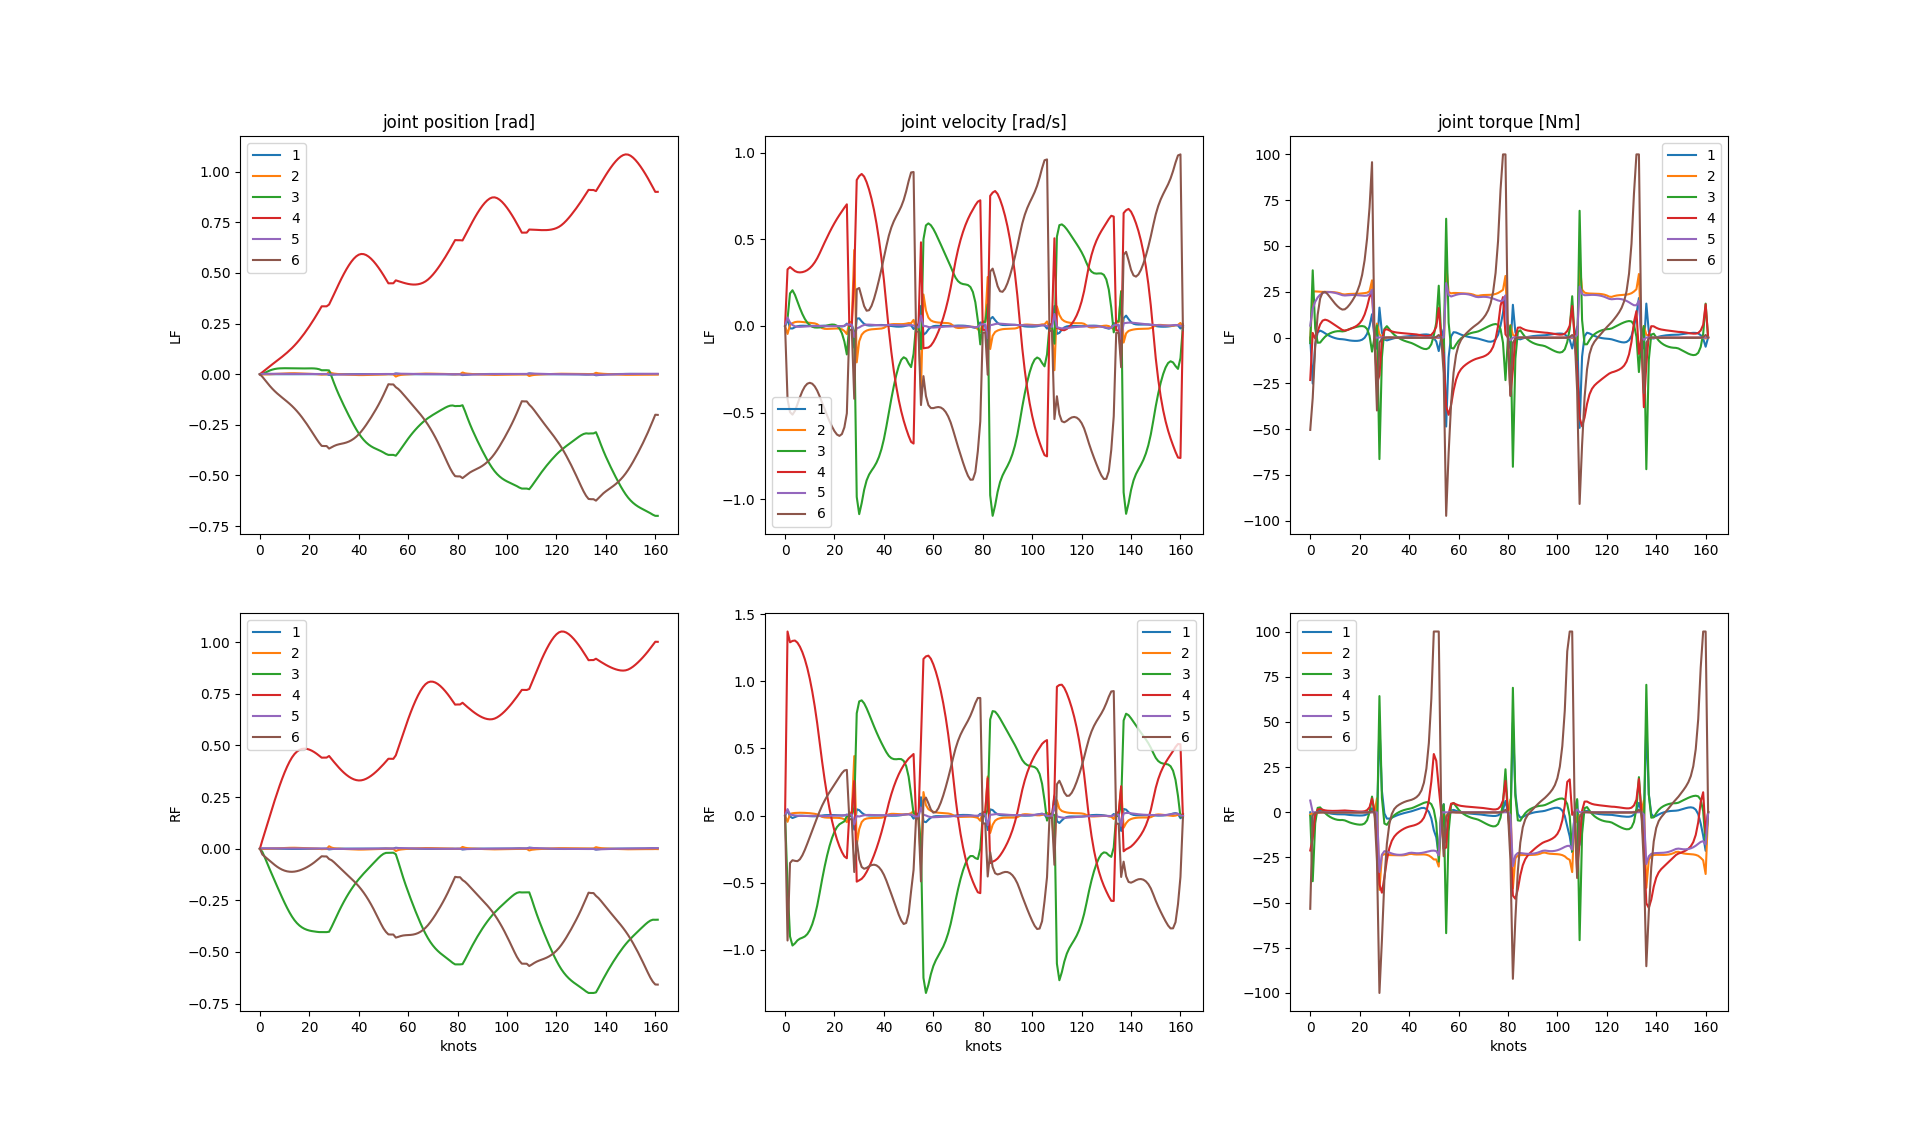
\includegraphics[width=1\linewidth]{Media/Crocoddyl/RH5/InitPoseVariants/RH5GaitInitZeroConfig_Solution.png}
  \caption{Solution for states and torques}.
\end{subfigure}
\begin{subfigure}{.8\textwidth}
  \centering
  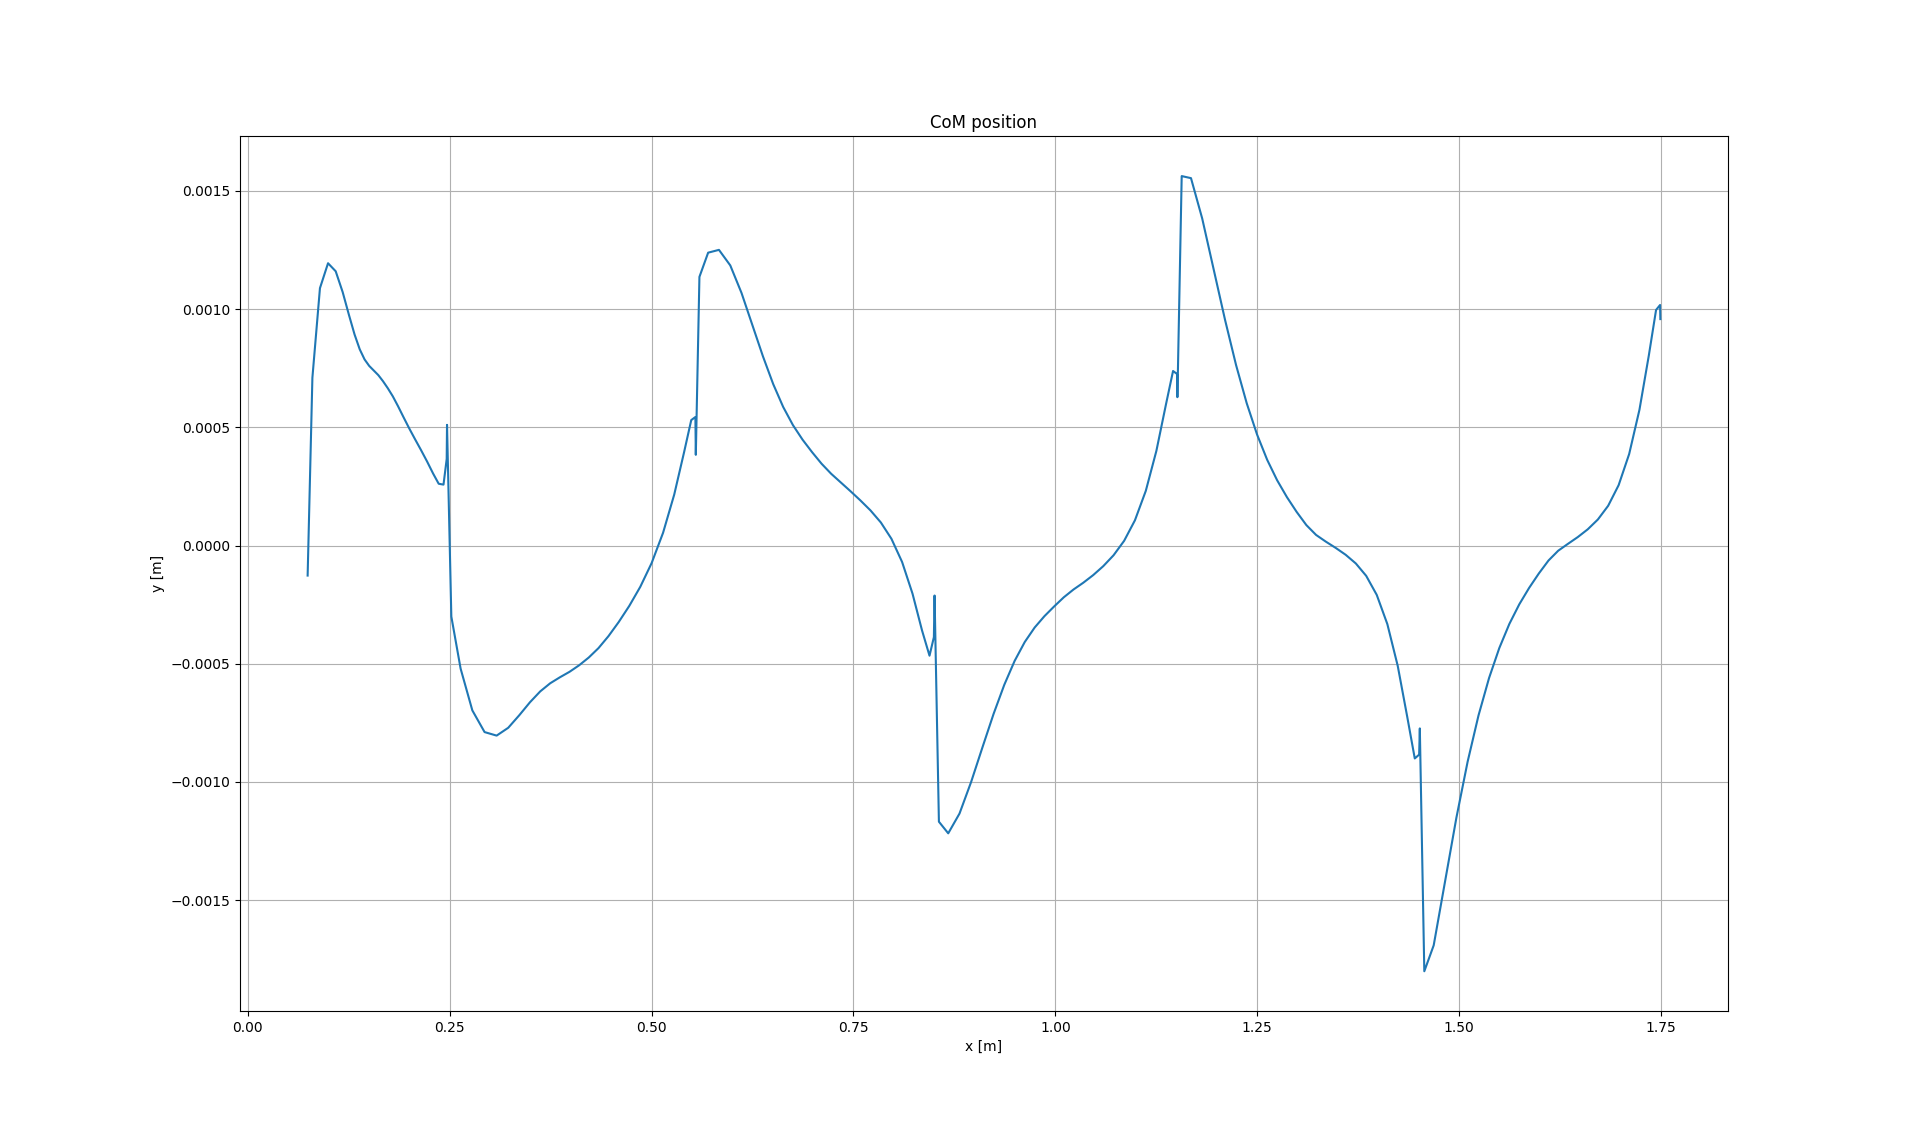
\includegraphics[width=1\linewidth]{Media/Crocoddyl/RH5/InitPoseVariants/RH5GaitInitZeroConfig_CoM.png}
\caption{CoM results.}
\end{subfigure}
\caption{Results for the full gait with initial pose \textbf{at} the zero configuration.}
\label{fig:rh5_init_at_zero}
\centering
\end{figure}

\begin{figure}[h!]
\centering
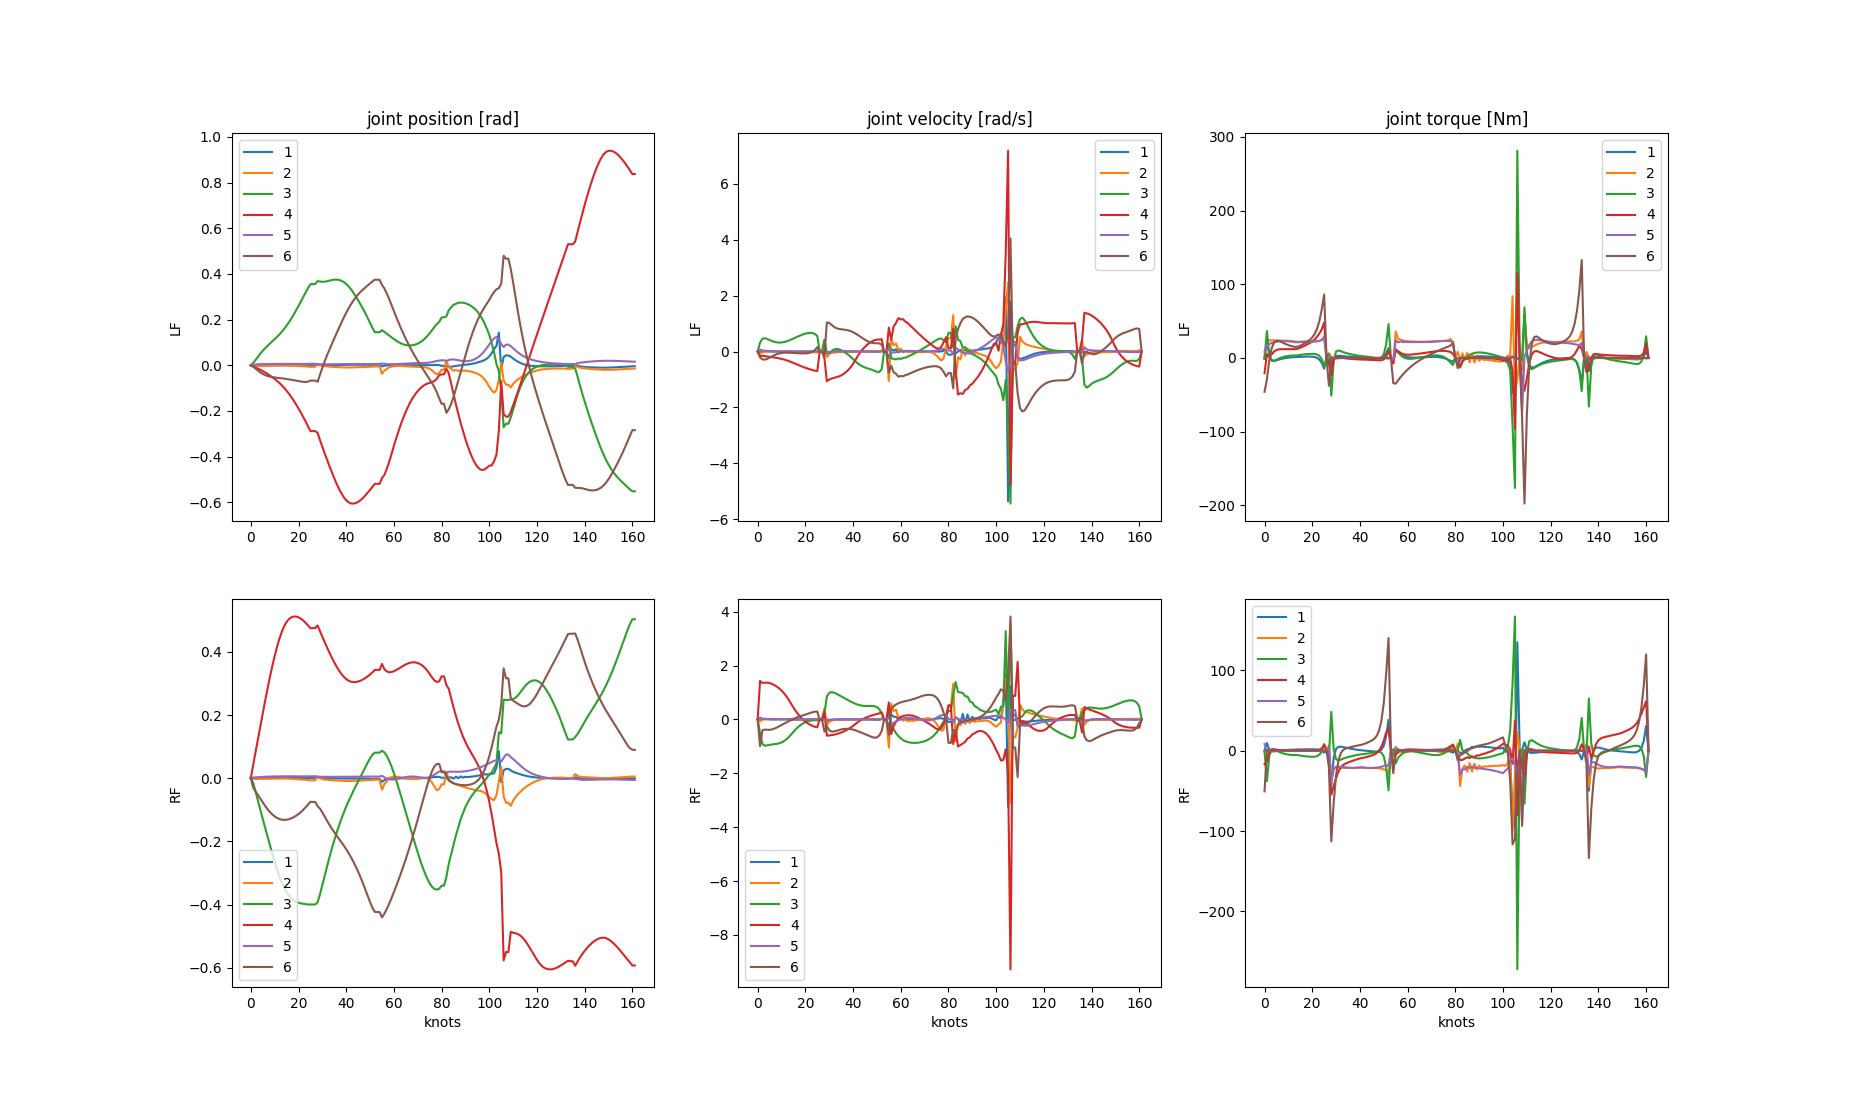
\includegraphics[width=1\linewidth]{Media/Crocoddyl/RH5/InitPoseVariants/RH5GaitInitZeroConfig_Solution_FailedSolver.png}
\caption{Another result for the full gait with initial pose \textbf{at} the zero configuration. The solution appears to be instable and would exceed the torque limits (see video).}
\label{fig:rh5_init_at_zero_failed_solver}
\end{figure}








 
\chapter{DRAKE - MIT CSAIL}
The second library we were interested in analyzing for its capabilites of generating bipedal walking patterns is Drake \cite{drake}. As it turned out, at the time of this work (spring 2020), Drake does not provide examples of legged locomotion anymore.  Because of limited time, such an example has not been implemented.

Consequently, this chapter starts with a brief introduction to Drake and then summarizes the work with some simple examples, especially passive dynamic walkers. The focus of this work has been shifted to enhance the results gained with the Crocoddyl library , as described in chapter \ref{chapter1}.  


\section{Introduction}
\subsection{Motivation}
Drake is a \textbf{C++ toolbox for}
\begin{itemize}
\item Analyzing the dynamics of robots
\item Building control systems for robots
\item Heavy emphasis on optimization-based design/analysis
\end{itemize}

Drake aims to \textbf{simulate} 
\begin{itemize}
\item Complex dynamics of robots (e.g. including friction, contact, aerodynamics etc.)
\item Emphasis on exposing the structure in the governing equations (sparsity, analytical gradients, polynomial structure, uncertainty etc.)
\item Making this information available for advanced planning, control, and analysis algorithms
\end{itemize}

Drake \textbf{provides}
\begin{itemize}
\item Python Interface
\item Implementation of state-of-the-art algorithms
\item Various examples
\end{itemize}

\subsection{Core Modules}
Drakes functionality is incorporated within several modules. This section gives a brief overview. 
\subsubsection{Modeling Dynamical Systems}
Drake uses a Simulink-inspired description of dynamical systems.

Includes basic building blocks (adders, integrators, delays, etc), physics models of mechanical systems, and a growing list of sensors, actuators, controllers, planners, estimators.
\subsubsection{Solving Mathematical Programs}
Drake's MathematicalProgram class is used to solve the mathematical optimization problem in the following form
$$min_{x} f(x) \quad s.t. x \in S$$
Depending on the formulation of the objective function $f$, and the structure of the constraint set $S$, Drake can solve the following categories of optimization problems
\begin{itemize}
\item Linear programming
\item Quadratic programming 
\item Nonlinear nonconvex programming
\item Semidefinite programming
\item Sum-of-squares programming
\item Mixed-integer programming
\end{itemize}
Drake \textbf{automatically} calls suitable solvers for each category of optimization problem.
\subsubsection{Multibody Kinematics and Dynamics}
\begin{itemize}
\item Drake's \textbf{constraint system} helps solve computational dynamics problems with algebraic constraints
\item Drake approximates real-world physical \textbf{contact} phenomena with a combination of geometric techniques and response models.
\end{itemize}

\section{How-To}
\subsection{Install}
Drake offers multiple ways of installation. This includes:
\begin{itemize}
\item Installation from Binaries
\item Installation from Source (using bazel)
\item Drake in Docker Containers
\end{itemize}
In this section some experiences for the installation from source and binaries are given. The choice mainly depends on if you want to use Drake via it's C++ or Python Interface. 
\subsubsection{Installation via Binaries}
Propably the easiest way to access the Drake functionalities is via \textbf{pydrake} (python bindings). In this case it should be sufficient to install the binaries of Drake and and access them from  a customized example directory, e.g. forked from the drake repo. 

For Ubuntu 18.04 the installation boils down to 
\begin{enumerate}
	\item Download and extract the latest version to your /opt 			directory:
	\begin{verbatim}
	curl -o drake.tar.gz https://drake-packages.csail.mit.edu/drake/		nightly/drake-latest-<platform>.tar.gz
	rm -rf /opt/drake
	tar -xvzf drake.tar.gz -C /opt
	\end{verbatim}
	\item Get the system dependencies:
	\begin{verbatim}
	/opt/drake/share/drake/setup/install_prereqs
	\end{verbatim}
	\item Add the python bindings to your PYTHONPATH environment 			variable:
	\begin{verbatim}
	export PYTHONPATH=/opt/drake/lib/python3.6/site-packages:$				{PYTHONPATH}
	\end{verbatim}
	\item Check if your installation was successful and that you can 	import pydrake:
	\begin{verbatim}
	python3 -c 'import pydrake; print(pydrake.__file__)'
	\end{verbatim}
\end{enumerate}
\subsubsection{Installation from Source Using Bazel}
If you instead prefer working directly on the \textbf{C++} examples or even want to contribute to the Drake library itself, an installation from source is recommended. 

Detailed instructions can be found here: \url{https://drake.mit.edu/from_source.html}.

Please note that the installation of Drake from source can take you \textbf{several hours}. 

\textbf{Issues during build process}

During installation from source I faced the following error message after a while:
\begin{verbatim}
Server terminated abruptly (error code: 14, error message: 'Socket closed'
\end{verbatim}
Maybe, this crash was caused by to less RAM (8GB). A workaround adapted from \url{https://stackoverflow.com/a/34399184} was to 
\begin{itemize}
\item Limit the number of parallel jobs and 
\item Limit the percentage of RAM Usage.
\end{itemize}
Finally, calling the build command with the following arguments was successfull:
\begin{verbatim}
CC=clang CXX=clang++ bazel build //... --ram_utilization_factor 30 --jobs=4
\end{verbatim}

\subsection{Run Python Examples}
Basically there are two kind of python examples provided:
\begin{itemize}
\item Encapsulated in a jupyter notebook (.jpnb): Interactively run the blocks
\item Pure python examples
\end{itemize}
The python examples can be found under the directory
\begin{verbatim}
/drake/bindings/pydrake/examples/multibody
\end{verbatim}
Within this directory, to run a \textbf{2D example} (using planar-scenegraph-visualizer):
\begin{verbatim}
python3 run_planar_scenegraph_visualizer.py
\end{verbatim}
If you instead want to run a \textbf{3D example} (using drake-visualizer):
In a first console open the visualizer from the binaries
\begin{verbatim}
/opt/drake/bin$ ./drake-visualizer
\end{verbatim}
Then, in a second console run (from your pydrake/examples/multibody directory again)
\begin{verbatim}
python3 cart_pole_passive_simulation.py
\end{verbatim}
to see a 3D visualization of the simulated dynamics of a cart-pole model.

\subsection{Additional Resources from MIT 6.832}\label{subsec:mit}
Additional to the examples provided within the drake, there is existing other useful material. The MITs Underactuated Robotics class \cite{mitx6.832web} offers a whole bunch of examples using pydrake. You can clone the repository with the course materials like this:
\begin{verbatim}
git clone https://github.com/RussTedrake/underactuated.git
sudo underactuated/scripts/setup/ubuntu/18.04/install_prereqs
export PYTHONPATH=`pwd`/underactuated:${PYTHONPATH}
\end{verbatim}


\section{Working with the Examples}
This section contains some applications of the Drake library within several examples. Herein, the focus lies on understanding the implementation, but additionally some insights about the system dynamics will be shown. 

Note that these examples are taken from Drake, but from the \href{http://underactuated.csail.mit.edu/underactuated.html}{MIT Underactuated Robotics class}. See section \ref{subsec:mit} for details on how to get the examples. The videos can all be found under \url{https://github.com/julesser/oc-frameworks/tree/master/OCFrameworks/Media/Drake}. 

\subsection{Cart-Pole}
One classic example of a simple underactuated system is the famous cart-pole model. The system has 2DOF $\theta, x$, where only the horizontal position $x$ is acutated. 
For further details on the system visit \url{http://underactuated.csail.mit.edu/acrobot.html#cart_pole}.
\subsubsection{Balancing around the upright using LQR}
The \href{http://underactuated.csail.mit.edu/lqr.html}{Linear Quadratic Regulator (LQR)} solves linear time-invariant system where the cost is described by a quadratic function.
An exemplary task can be to stabilize the uprgith position of the pendulum from initial conditions.

\subsubsection{Trajectory Optimization using Direct Collocation}
From a methodology point of view, this example is interesting for our research and therefore will be explained in a bit more detail. The resulting dynamic up-swinging and and stabilization can best be seen in the \href{https://raw.githubusercontent.com/julesser/oc-frameworks/master/OCFrameworks/Media/Drake/ExSimple/CartpoleTrajOptDirCol.mp4}{videos}, while the optimal force solution presented in Figure \ref{fig:cart-pole}.
\begin{enumerate}
\item Load and build the dynamic model (\textit{plant+context})
\begin{verbatim}
plant = MultibodyPlant(time_step=0.0)
scene_graph = SceneGraph()
plant.RegisterAsSourceForSceneGraph(scene_graph)
file_name = FindResource("models/cartpole.urdf")
Parser(plant).AddModelFromFile(file_name)
plant.Finalize()
context = plant.CreateDefaultContext()
\end{verbatim}
\item Setup the optimization problem with discrete, uniform time steps (i.e. knots)
\begin{verbatim}
dircol = DirectCollocation(
    plant,
    context,
    num_time_samples=21,
    minimum_timestep=0.1,
    maximum_timestep=0.4,
    input_port_index=plant.get_actuation_input_port().get_index())
dircol.AddEqualTimeIntervalsConstraints()
\end{verbatim}
\item Specify the initial and terminal state via constraints
\begin{verbatim}
initial_state = (0., 0., 0., 0.)
dircol.AddLinearConstraint(dircol.initial_state() == initial_state)
final_state = (0., math.pi, 0., 0.)
dircol.AddLinearConstraint(dircol.final_state() == final_state)
\end{verbatim}
\item For each running knot, penalize actuator effort. For the terminal state, penalize the total time consumped.
\begin{verbatim}
R = 10  # Cost on input "effort".
u = dircol.input()
dircol.AddRunningCost(R * u[0]**2)
dircol.AddFinalCost(dircol.time())
\end{verbatim}
\item Generate a piecewise-polynomial function and use it as initial guess
\begin{verbatim}
initial_x_trajectory = PiecewisePolynomial.FirstOrderHold(
    [0., 4.], np.column_stack((initial_state, final_state)))  
dircol.SetInitialTrajectory(PiecewisePolynomial(), initial_x_trajectory)
\end{verbatim}
\item Solve the trajectory optimizaton problem
\begin{verbatim}
result = Solve(dircol)
\end{verbatim}
\end{enumerate}

\begin{figure}[h!]
\centering
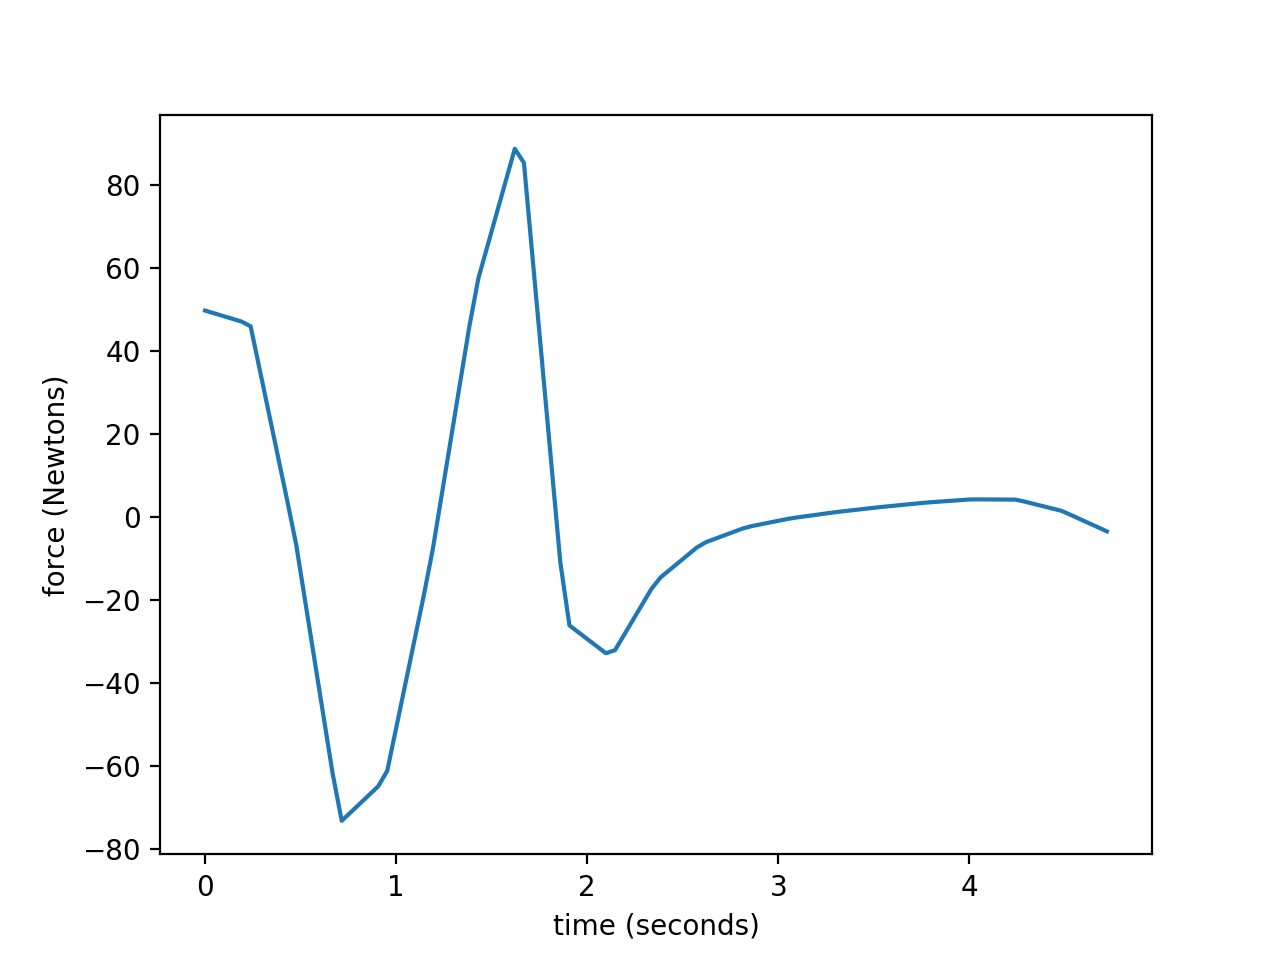
\includegraphics[width=.7\linewidth]{Media/Drake/ExSimple/CartPoleTrajOptDirCol_Solution.png}
\caption{Resulting optimal horizontal force from trajectory optimization of the up-swining and stabilization for the cart-pole.}
\label{fig:cart-pole}
\end{figure}

\subsection{Passive Dynamic Walkers}
Although there currently are no highly-articulated robots found in the Drake examples, it does provide some classic examples of simplified locomotion models. 

\subsubsection{Rimless Wheel}
Simulating the simple dynamics of the rimless wheel model rolling down a declining slope, an continous limit cycle emerges (see Figure \ref{fig:rimlessWheel}).
\begin{figure}[h!]
\centering
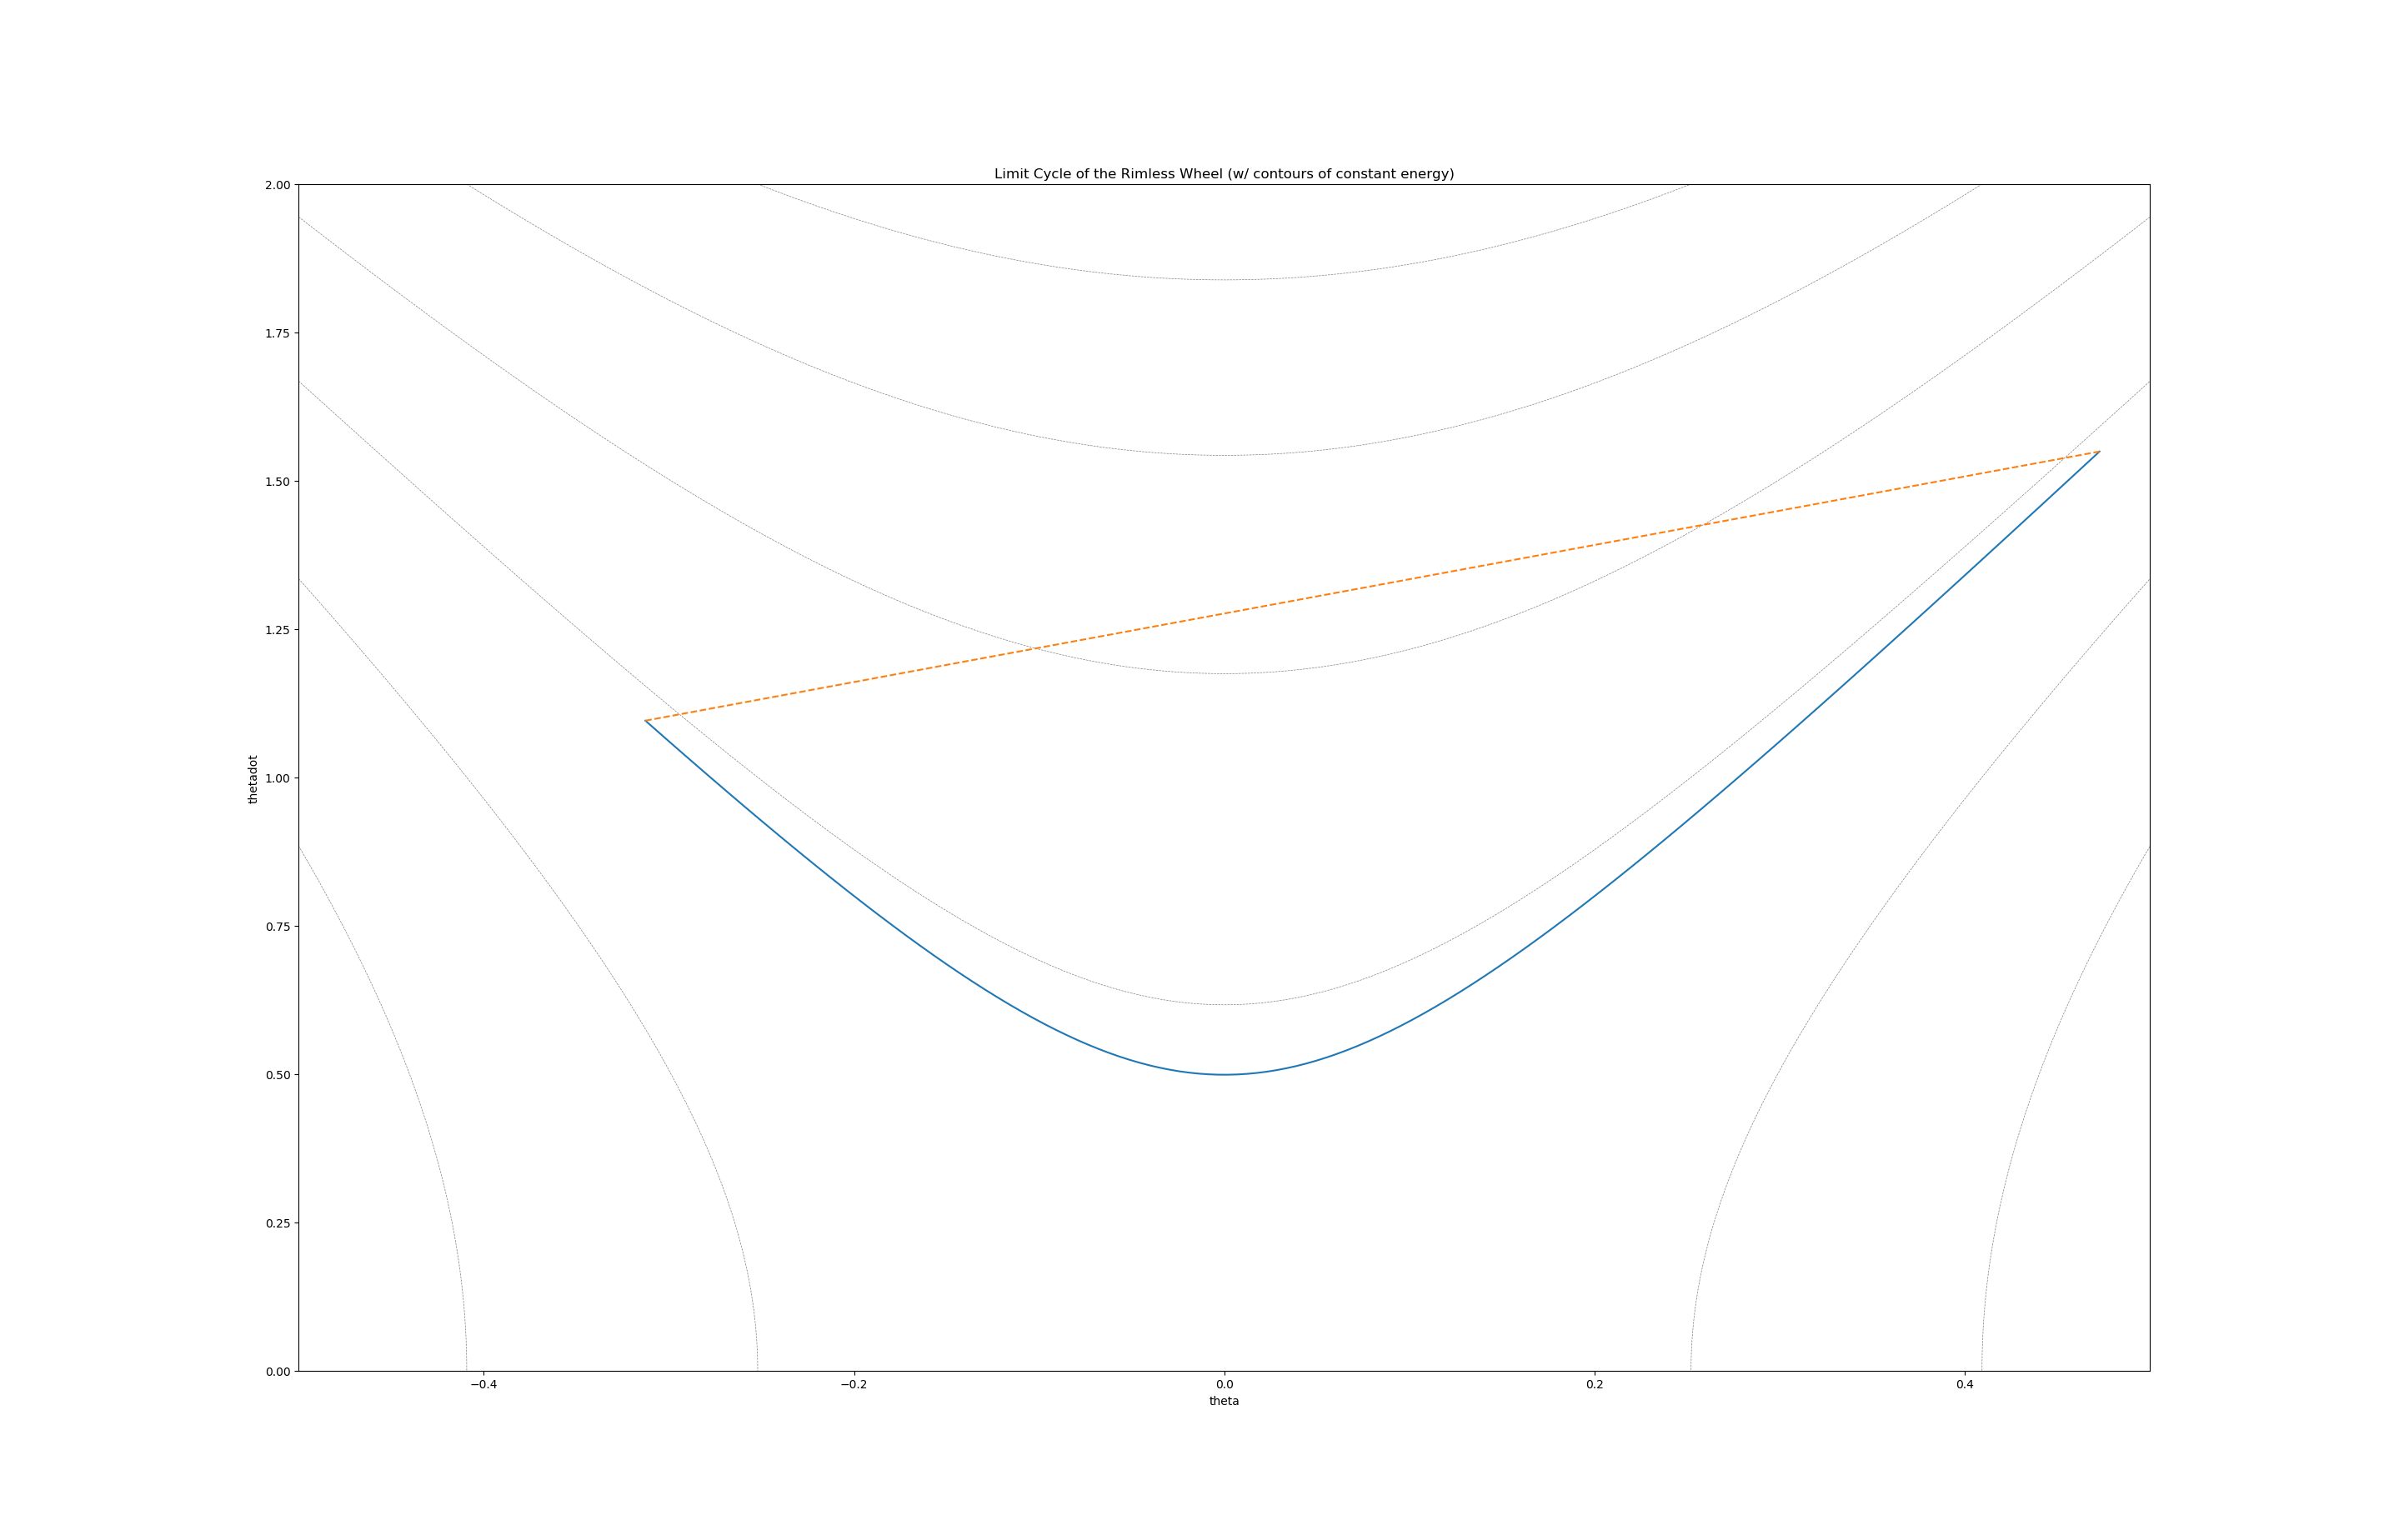
\includegraphics[width=1\linewidth]{Media/Drake/ExSimpleWalking/RimlessWheelDirCol_LimitCycle.png}
\caption{Results for an energy-optimal limit cycle for the rimless wheel using direct collocation trajectory optimization.}
\label{fig:rimlessWheel}
\end{figure}

\subsubsection{Compass Gait}
The compass gait is a simple bipedal walking model containing two links and three pointmasses. For further details on the system visit \url{http://underactuated.csail.mit.edu/simple_legs.html#section2}. 

Simulating the system dynamics for a declining slope results in periodic motions (see Figure \ref{fig:compassGait}).
\begin{figure}[h!]
\centering
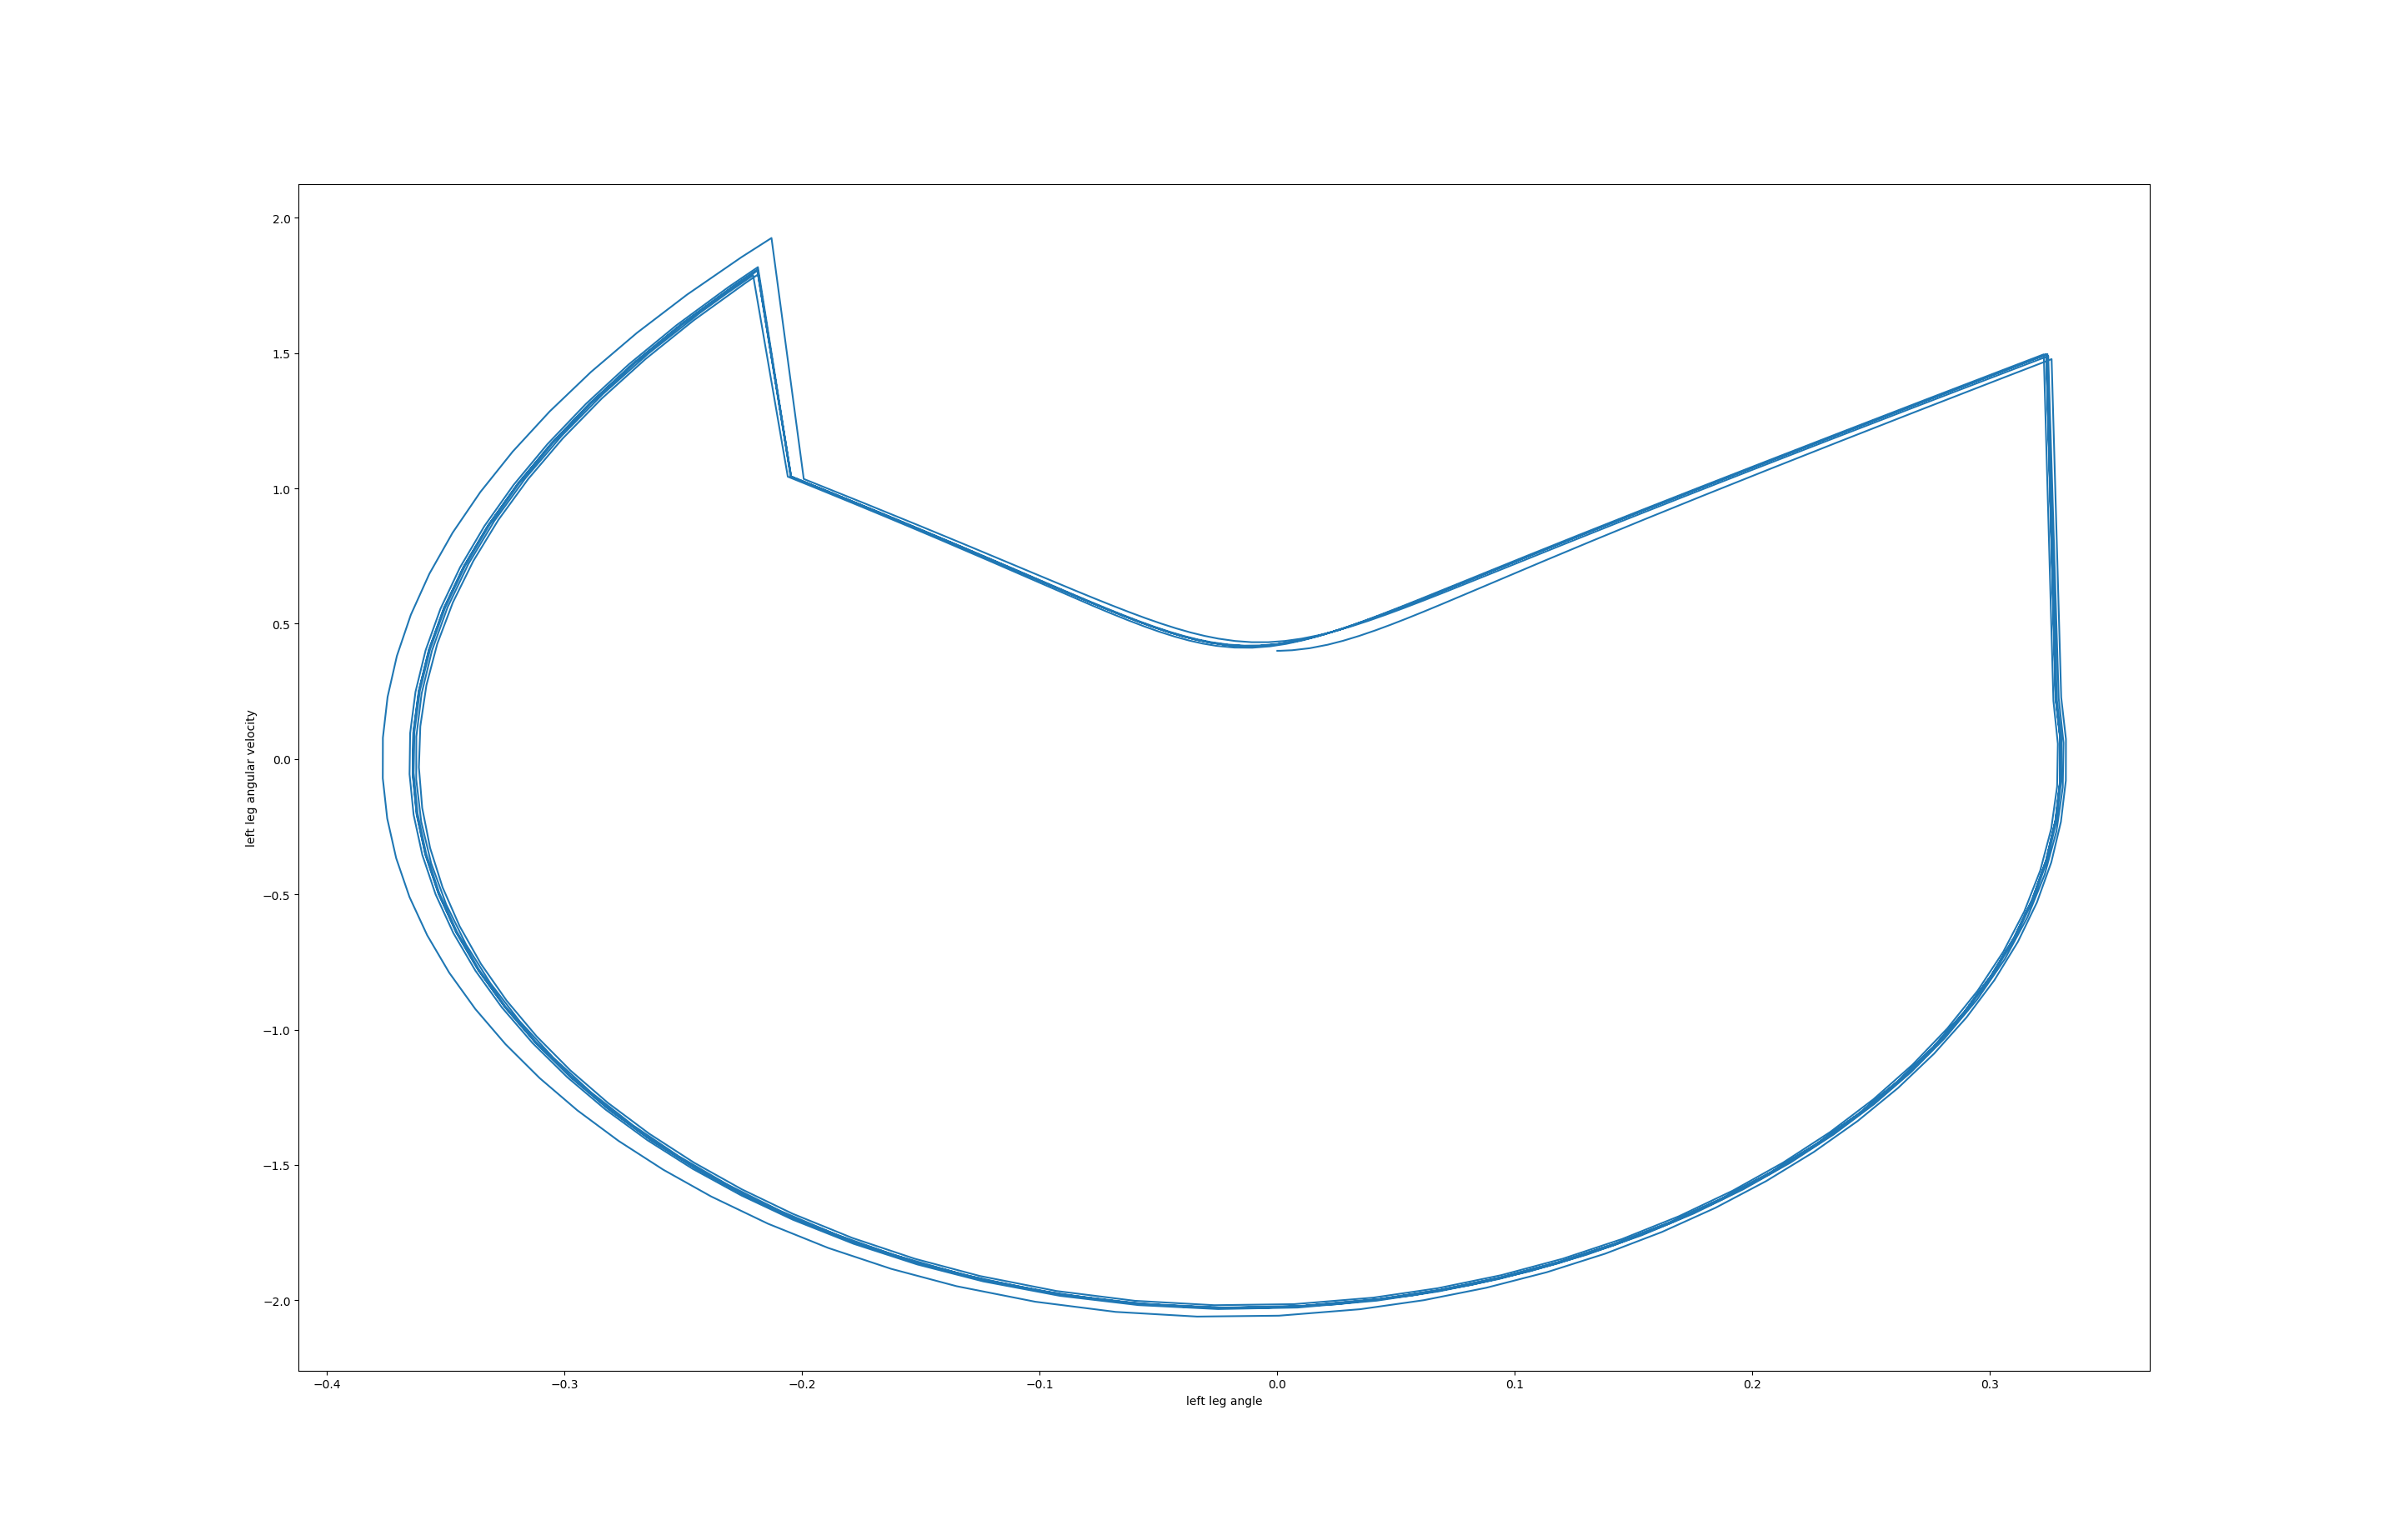
\includegraphics[width=1\linewidth]{Media/Drake/ExSimpleWalking/CompassGait_PhasePlot.png}
\caption{Resulting phase plot of the compass gait reveals periodic orbits.}
\label{fig:compassGait}
\end{figure}



\chapter{Lecture 3/4: Dynamic Programming}\label{lecture3}
\section{Control as Optimization}
\begin{itemize}
\item The big idea is to formulate control design as an optimization problem.
\item Given a trajectory $x(.),u(.)$ we want to assign a score (scalar) to decribe the performance.
\item Additionally we can set constraints in order to exclude trajectories that exceed certain limits (e.g. control limit $\abs{u(t)}<=1$).
\item The goal is to find a control policy $u=\Pi(t,x)$ that optimizes that score!
\item When solving optimal control problems, one most often needs numerical approximation.
\end{itemize}
The strengths of Optimal Control are that it
\begin{itemize}
\item is a very general approach; it can be applied to fully/underactuated, linear/nonlinear systems,
\item contains an very intuitive approach by describing just the goal and some constraints 
\item works very well with numerical approximation.

\end{itemize}
 
 
\section{Example: Double Integrator}\begin{itemize}
\item Very simple example that can be solved without numerical approximation.
\item Consists of "brick of ice" on a flat floor
\item Goal: Go to origin as fast as possible
\end{itemize}
Easiest case: Formulate optimal control as "Bang-Bang". Accelerate (full throttle) then slam on the brakes.


\section{DDP: Discrete Time Space - Optimal Control as Graph Search}
For systems with a finite, discrete set of states and a finite, discrete set of actions, dynamic programming also represents a set of very efficient numerical algorithms which can compute optimal feedback controllers.

Cost function
$$one-step cost: g(s,a)$$
$$total cost: \sum_{n=0}^{\infty} $$
Key idea: Additive cost 
$$\int_0^T \ell(x(t),u(t)) dt,$$
There are existing numerous possibilities on how to design the cost function:
\begin{itemize}
\item Min-time: $g(s,a) = 1 "if" s~=s_{goal}; 0 if otherwise$
\item Quadratic cost: $g(x,u)=x^{T}x+u^{T}u$
\end{itemize}
There are many algorithms for finding (or approximating) the optimal path from a start to a goal on directed graphs. In dynamic programming, the key insight is that we can find the shortest path from every node by solving recursively for the optimal cost-to-go (the cost that will be accumulated when running the optimal controller) from every node to the goal.
Recursive form of the optimal control problem:
\begin{equation} \hat{J}^*(s_i) \Leftarrow \min_{a \in A} \left[ \ell(s_i,a) +
    \hat{J}^*\left({f(s_i,a)}\right) \right]
    \end{equation}
If we know the optimal cost-to-go, then it's easy to extract the optimal policy:
\begin{equation} \pi^{*}(s_i) = argmin_a
    \left[ \ell(s_i,a) + J^*\left( f(s_i,a) \right) \right].
\end{equation}

Limitations:
\begin{itemize}
\item Accuracy for continuous systems (discretisation error)
\item Scaling (curse of dimensionality)
\item Assumes full state information: Absolutely not necessary to know everything
\end{itemize}


\section{DDP: Continuous Time Space}
\subsection{The Hamilton-Jacobi-Bellman Equation}
An analogous set of conditions can be found in the continuous time space. For a system
$$ \dot{x}=f(x,u)$$
and an infinite-horizon additive cost
$$\int_0^\infty l(x,u)dt $$
we have
$$0=min_u \begin{bmatrix}
l(x,u)+\dfrac{\delta J^*}{\delta x}f(x,u)
\end{bmatrix}$$
$$\Pi^\star=argmin_u\begin{bmatrix}
l(x,u)+\dfrac{\delta J^*}{\delta x}f(x,u)
\end{bmatrix}$$








\chapter{Lecture 5-7: Acrobots, Cart-poles, and Quadrotors}
\section{Introduction}
So far we have covered the following topics:
\begin{itemize}
\item Manipulator Equations
\item Feedback Linearization
\item Optimal Control
\item Value Iteration (Algorithm for DDP in discrete time)
\end{itemize}
After introducing basics of "classic" non-linear control, we started thinking about control as optimization.

In this chapter the most simple standard models for underactuated robots are introduced. These low-dimensional systems are supposed to capture the essence of the problem without all the real-world complexity of advanced systems. 

\section{System Dynamics: Manipulator Equations}
The Acrobot is a simple underactuated system since it has two DoF. But, in comparison to the double pendulum, it only has one actuator at the elbow so that 
$\myM{B}=\begin{bmatrix} 0 & 1 \end{bmatrix}^T $.
Manipulator Equations: 
\begin{equation*}
\myM{M}(\myM{q})\myM{\ddot{q}}+\myM{C}(\myM{q,\dot{q}})\myM{\dot{q}}=\tau_g(\myM{q})+\myM{Bu}.
\end{equation*}
The goal is to swing-up and balance while satisfying some torque limits. One possible approach to solve this problem is using \textit{value iteration}. But the grids would have to be very fine, in order to get a good solution. There are better tools to solve this problem: LQR!


\section{Balancing for Acrobot and Cart-Pole}
For both the Acrobot and the Cart-Pole systems, we will begin by designing a linear controller which can balance the system when it begins in the vicinity of the unstable fixed point. To accomplish this, we will linearize the nonlinear equations about the fixed point, examine the controllability of this linear system, then using linear quadratic regulator (LQR) theory to design our feedback controller.

What we'll do to accomplish the balancing: 
\begin{enumerate}
\item Linearizing the manipulator equations
\item Check controllability of linear systems
\item Use LQR to design a feedback controller
\end{enumerate}
\subsection{Recap: LQR}
We have a linear time-invariant system in state-space form
\begin{equation*} 
\myM{\dot{x}}=\myM{Ax}+\myM{Bu},
\end{equation*}
the cost function is 
\begin{equation*} 
J = \int_0^{\infty}[\myM{x}^T\myM{Qx}+\myM{u}	^T\myM{Ru}]dt,
\end{equation*}
and the goal is to find the optimal cost-to-go function $J^\star(\myM{x})$ which satisfies the Hamilton-Jacobi-Bellman equation.
This yields 
\begin{equation*} 
J^\star(\myM{x}) = \myM{x}^T\myM{Sx}
\end{equation*}
and the optimal control policy 
\begin{equation*} 
\myM{u}^\star=\myM{Kx}.
\end{equation*}
In the end, this means you get the control policy and the cost-to-go function by
\begin{equation*} 
\myM{K,S}=LinearQuadraticRegulator(\myM{A}, \myM{B}, \myM{Q}, \myM{R}).
\end{equation*}
So you set $\myM{A}, \myM{B}$ from linearization and choose $\myM{Q}, \myM{R}$ and receive an optimal controller.

\subsection{Linearization of Nonlinear Systems}
\textbf{Problem:} Our systems are non-linear! How shall we apply Linear-Quadratic Control?!

\textbf{Solution:} We linearize our system around a specific fixed point.

But we need to be aware that our linearization only is valid within a certain area around this point. If you go to far away from it, the non-linearity overwhelms your solution. 

One Optimal Control Algorithm therefore is to combine multiple LQR Controllers that treat all relevant fixed points in order to handle the relevant workspace. 

\section{Throwback: Hand-Designed Control}
\begin{itemize}
\item Optimal control is a powerful framework for solving control problems via optimization.
\item Solving OC problems for non-linear systems is hard!
\item Sometimes we would be happy to just have any controller (And sometimes they turn out to be even better).
\item But how can we proof this "hand-designed" are any good? 
\section{Partial Feedback Linearization (Acrobot,Cart-pole)}
Although we cannot always simplify the full dynamics of the system, it is still possible to linearize a portion of the system dynamics. The technique is called partial feedback linearization.
\begin{itemize}
\item \textit{Collocated} PFL: A controller which linearizes the dynamics of the \textit{actuated} joints
\item \textit{Non-Collocated} PFL: A controller which linearizes the dynamics of the \textit{unactuated} joints
\end{itemize}
One of the most important lessons from partial feedback linearization, is the idea that if you have m actuators, then you basically get to control exactly m quantities of your system.

-> We proof that they are stable. 
\end{itemize}

\section{Swing-Up Control: Energy Shaping (Acrobot,Cart-pole)}
If we seek to design a nonlinear feedback control policy which drives the simple pendulum from any initial condition to the unstable fixed point, a very reasonable strategy would be to use actuation to regulate the energy of the pendulum to place it on this homoclinic orbit, then allow the system dynamics to carry us to the unstable fixed point.

This idea turns out to be a bit more general than just for the simple pendulum. As we will see, we can use similar concepts of `energy shaping' to produce swing-up controllers for the acrobot and cart-pole systems. It's important to note that it only takes one actuator to change the total energy of a system.

The basic Idea for the swing-up control is to
\begin{enumerate}
\item Use collocated PFL to simplify the dynamics
\item Use energy shaping to regulate the pendulum to its homoclinic orbit
\item Add a few terms to make sure that the cart stays near the origin
\end{enumerate}


\section{Differential Flatness (Quadrotors)}
The task we'll consider for quadrotors is trajectory optimization:

How can you find a feasible trajectory through state space for the quadrotor, even if there are obstacles to avoid that are only known at runtime? 

Trajectory design, and especially trajectory optimization, is a big idea that we will explore more thoroughly later in the text. But there is one idea that I would like to present here, because in addition to being a very satisfying solution for quadrotors, it is philosophically quite close to the idea of partial feedback linearization. That idea is called differential flatness.

\begin{itemize}
\item Similar idea as PFL: Given a trajectory of m (number of actuators) coordinates. 
\item Then, the control input and all left states can be guessed
\item Condition: Trajectory needs to be four-times differentiable
\end{itemize}

2D-Quadrotor Example (m=2): Given x,y of trajectory, guess resulting jaw and control input.

3D-Quadrotor Example (m=4): Given x,y,z,jaw guess roll, pitch and control for all motors.


\chapter{Lecture 8/9: Lyapunov Analysis}
Optimal control provides a powerful framework for formulating control problems using the language of optimization. But solving optimal control problems for nonlinear systems is hard! In many cases, we don't really care about finding the optimal controller, but would be satisfied with any controller that is guaranteed to accomplish the specified task. In many cases, we still formulate these problems using computational tools from optimization, and in this chapter we'll learn about tools that can provide guaranteed control solutions for systems that are beyond the complexity for which we can find the optimal feedback.


\section{Lyapunov Functions}
\subsection{Optimization Crash Course}
\begin{itemize}
\item Goal: Find $x_{min}$ for an objective (cost) function considering a set of (in/equality-) constraints
\item Popular objective functions:
\begin{itemize}
\item Convex quadratic cost (least squares)
\item Linear cost
\end{itemize}
\item Convex optimization builds on convex cost functions or a convex set
\end{itemize}

\subsection{Introduction}
Lyapunov functions generalize the notion of an energy function to more general systems, which might not be stable in the sense of some mechanical energy. If I can find any positive function, call it$V(\myM{x})$, that gets smaller over time as the system evolves, then I can potentially use $V$ to make a statement about the long-term behavior of the system. $V$is called a Lyapunov function. 


\section{Lyapunov Analysis with Convex Optimization}
In this section, we'll look at some computational approaches to verifying the Lyapunov conditions, and even to searching for (the coefficients of) the Lyapunov functions themselves.
\subsection{Lyapunov Analysis for Linear Systems}
Imagine you have a linear system
$\myM{\dot{x}}=\myM{Ax},$
and can find a Lyapunov function
$$V(\myM{x})=\myM{x}^T\myM{Px}, \myM{P}=\myM{P}^T>0,$$
which also satisfies
$$\myM{\dot{V}(x)}=\myM{x}^T\myM{PAx}+\myM{x}^T\myM{A}^TPx<0.$$
Then the origin is globally asymptotically stable.

\subsection{Lyapunov Analysis as a Semi-definite Program (SDP)}
Lyapunov analysis for linear systems has an extremely important connection to convex optimization. In particular, we could have also formulated the Lyapunov conditions for linear systems above using semi-definite programming (SDP). Semidefinite programming is a subset of convex optimization -- an extremely important class of problems for which we can produce efficient algorithms that are guaranteed find the global optima solution 
\subsection{Sums-of-squares Optimization}
It turns out that in the same way that we can use SDP to search over the positive quadratic equations, we can generalize this to search over the positive polynomial equations.


\section{Lyapunov Analysis for Estimating Regions of Attraction}
There is another very important connection between Lyapunov functions and the concept of an invariant set: any sub-level set of a Lyapunov function is also an invariant set. This gives us the ability to use sub-level sets of a Lyapunov function as approximations of the region of attraction for nonlinear systems.

Now we have arrived at the tool that I believe can be a work-horse for many serious robotics applications. Most of our robots are not actually globally stable (that's not because they are robots -- if you push me hard enough, I will fall down, too), which means that understanding the regions where a particular controller can be guaranteed to work can be of critical importance.

Sums-of-squares optimization effectively gives us an oracle which we can ask: is this polynomial positive for all x? To use this for regional analysis, we have to figure out how to modify our questions to the oracle so that the oracle will say "yes" or "no" when we ask if a function is positive over a certain region which is a subset of R. That trick is called the S-procedure. It is closely related to the Lagrange multipliers from constrained optimization, and has deep connections to "Positivstellensatz" from algebraic geometry.


\chapter{Lecture 10: Trajectory Optimization}
\section{Recap: What Did We Cover so Far?}
The\textbf{ overall goal} is to specify complex behaviors with simple objective functions, letting the dynamics and constraints on the system shape the resulting feedback controller.

But the computational tools that we've provided so far have been \textbf{limited} in some important ways:
\begin{itemize}
\item \textbf{Dynamic programming} involves putting a mesh over the state space 

-> Stuck in low-dimensional systems.
\item \textbf{LQR} + \textbf{Linearization} around an operating point; applicable to high-dimensional systems 

-> Linearization only valid for a certain region of the state space
\item \textbf{Lyapunov Analysis via SDP/SOS} softens the requirements by not searching for the optimal controller, but only searching for stability. It does so for non-linear systems and all $\myM{x}$ (whole state-space).

-> No controller actually synthesised + somehow limited to simple Lyapunov functions (quadratic, polynomials etc) which might limit the control design  
\end{itemize}
But we have not yet provided any real computational tools for approximate optimal control that work for high-dimensional systems beyond the linearization around a goal. That is precisely the goal for this chapter.

\textbf{Q:} How can we handle complex systems?

\textbf{A:} We ask not for all states (like in Lyapunov Analysis), instead only the relevant ones!
\begin{itemize}
\item For the beginning: Consider only one single initial condition!
\item Maybe some $x_0$ in the neighbourhood are also good
\item Represent the solution as a trajectory,  $\myM{x}(t), \myM{u}(t)$, typically defined over a finite interval (instaed of feedback control function)
\item \textbf{This means:} 
\begin{enumerate}
\item We define only a single trajectory $\myM{u}(t)$, 
\item Search for optimal states $\myM{x}$ and control inputs $\myM{u}$,
\item To follow this trajectory as good as possible!
\end{enumerate}
\end{itemize}


\section{Problem Formulation}
\begin{itemize}
\item Min over a finite trajectory over time $\myM{u}(\cdot)$
\item Initial conditions $x(0)$ are fixed and known
\end{itemize}
\begin{align*}
\min_{\myM{u}(\cdot)} \quad &
\int_{t_0}^{t_f} \ell(\myM{b}(t),\myM{b}(t)) dt \\ \text{subject to} \quad &
\forall t, \dot{\myM{x}}(t)=f(\myM{x}(t),\myM{u}(t)), \\
& \myM{x}(t_0)=x_0
\end{align*}


\section{Computational Tools for Nonlinear Optimization}
Intro 
\section{Trajectory Optimization as a Nonlinear Program}
As written above, the optimization above is an optimization over continuous trajectories. In order to formulate this as a numerical optimization, we must parameterize it with a finite set of numbers. 

Different approaches on how to do this, are:
\begin{itemize}
\item Idea 1). \textbf{Direct Transcription}: Fix breakpoints at even intervals $dt$ and use Euler integration. Decision variables are $x,n$ 
\item Idea 2.) \textbf{Direct Shooting Methods} - Idea: Destrict decision variables to only $u$ and and compute $x$ ourselves by knowing $x_0$ and $u(\cdot)$ via the simple forward dynamics
$$x[t=0] = x_0$$
$$x[1]=Ax_0+Bu[0]$$
$$x[2]=A\cdot(x[1]=Ax_0+Bu[0])+Bu[0]$$
$$...$$
\item Idea 3.) \textbf{Direct Collocation:} Assume first-order polynomial for $\myM{u}(t)$ and cubic polynomial $\myM{x}(t)$.
\end{itemize}


\section{Pontryagins's Minimum Principle}


\section{Trajectory Stabilization: Local Trajectory Feedback Design}
What we want is to move robots in the real world. Therefore it is not useful to have only one exact trajectory, but we need to allow the robot to move in a \textbf{band around our target trajectory}. 

\textbf{Idea}: Locally linearize around our points from the trajectory, so that we can apply tools from linear control again.

\subsection{Linear Model-predictive Control}
Locally stabilizes a \textbf{constrained} system.
\subsection{Time-varying LQR}
Locally stabilizes $\myM{x}_0(t), \myM{u}_0(t)$

\section{Iterative LQR}



  



%\chapter{Lecture 12/13: Simple Models of Walking and Running}
In this chapter we'll introduce some of the simple models of walking and robots, the control problems that result, and a very brief summary of some of the control solutions described in the literature. Compared to the robots that we have studied so far, our investigations of legged locomotion will require additional tools for thinking about limit cycle dynamics and dealing with impacts.


\section{Limit Cycles}
In many of the systems that we have studied so far, we have analyzed the stability of a fixed-point, or even an (infinite-horizon) trajectory. For walking systems the natural equivalent is to talk about the stability of periodic solutions -- a fixed "gait" is a cycle that repeats footstep after footstep. So we begin our discussion with a discussion of the stability of a cycle.
A limit cycle is an asymptotically stable or unstable periodic orbit. One of the simplest models of limit cycle behavior is the Van der Pol oscillator.
\subsection{Poincare Maps}


\section{Simple Models of Walking}
\subsection{The Rimless Wheel}
The most elementary model of passive dynamic walking, first used in the context of walking by, is the rimless wheel. This simplified system has rigid legs and only a point mass at the hip as illustrated in the figure above. To further simplify the analysis, we make the following modeling assumptions
\begin{itemize}
\item No slip
\item Collisions are inelastic and impulsive (no bouncing)
\item No double support
\end{itemize}
\subsection{The Compass Gait}
\subsection{The Kneed Walker}


\section{Simple Models of Running}
\subsection{The Spring-Loaded Inverted Pendulum}
\subsection{The Planar Monopod Hopper}


\section{A Simple Model That Can Walk and Run}













































\pagebreak
% Adding a bibliography if citations are used in the report
\bibliographystyle{plain}
\bibliography{../commonBibFile.bib}
% Adds reference to the Bibliography in the ToC
\addcontentsline{toc}{chapter}{\bibname}

\pagebreak



\end{document}
